%%%%%%%%%%%%%%%%%%%%%%%%%%%%%%%%%%%%%%%%%%%%%%%%%%%%%%%%%%%%%%%%%%%%%%%%%%%%%
% parámetros para configurar el formato del código en los entornos lstlisting
%%%%%%%%%%%%%%%%%%%%%%%%%%%%%%%%%%%%%%%%%%%%%%%%%%%%%%%%%%%%%%%%%%%%%%%%%%%%%
\lstset{ %
    backgroundcolor=\color{white},   % choose the background color; you must add \usepackage{color} or \usepackage{xcolor}
    basicstyle=\footnotesize,        % the size of the fonts that are used for the code
    breakatwhitespace=false,         % sets if automatic breaks should only happen at whitespace
    breaklines=true,                 % sets automatic line breaking
    captionpos=b,                    % sets the caption-position to bottom
    commentstyle=\color{mygreen},    % comment style
    deletekeywords={...},            % if you want to delete keywords from the given language
    %escapeinside={\%*}{*)},          % if you want to add LaTeX within your code
    %extendedchars=true,              % lets you use non-ASCII characters; for 8-bits encodings only, does not work with UTF-8
    %frame=single,	                % adds a frame around the code
    keepspaces=true, keywordstyle=\color{blue}, language=[ANSI]C, % keeps spaces in text, useful for keeping indentation of code (possibly needs columns=flexible)% keyword style% the language of the code
    %otherkeywords={*,...},           % if you want to add more keywords to the set
    numbers=left, numbersep=5pt, numberstyle=\tiny\color{mygray},
    rulecolor=\color{black}, showspaces=false, showstringspaces=false,
    showtabs=false, stepnumber=1, stringstyle=\color{mymauve}, tabsize=2,
    title=\lstname, morecomment=[s]{/*}{*/} }% where to put the line-numbers; possible values are (none, left, right)% how far the line-numbers are from the code% the style that is used for the line-numbers% if not set, the frame-color may be changed on line-breaks within not-black text (e.g. comments (green here))% show spaces everywhere adding particular underscores; it overrides 'showstringspaces'% underline spaces within strings only% show tabs within strings adding particular underscores% the step between two line-numbers. If it's 1, each line will be numbered% string literal style% sets default tabsize to 2 spaces% show the filename of files included with \lstinputlisting; also try caption instead of title

\lstdefinelanguage{PythonUTF8}[]{Python}{
literate={á}{{\'a}}1 {é}{{\'e}}1 {í}{{\'i}}1 {ó}{{\'o}}1 {ú}{{\'u}}1
{Á}{{\'A}}1 {É}{{\'E}}1 {Í}{{\'I}}1 {Ó}{{\'O}}1 {Ú}{{\'U}}1
{ñ}{{\~n}}1 {Ñ}{{\~N}}1
}

\definecolor{mygreen}{rgb}{0,0.6,0}
\definecolor{mygray}{rgb}{0.5,0.5,0.5}
\definecolor{mymauve}{rgb}{0.58,0,0.82}

\chapter{Diseño e implementación} % Main chapter title

\label{Chapter3} % Change X to a consecutive number; for referencing this chapter elsewhere, use \ref{ChapterX}

Este capítulo describe el diseño y la implementación del sistema de monitoreo y
control de invernaderos. Se detallan los componentes principales del sistema,
las decisiones de diseño tomadas y los pasos seguidos para su implementación.

%----------------------------------------------------------------------------------------
%	SECTION 1
%----------------------------------------------------------------------------------------
\section{Arquitectura del sistema}

La figura \ref{fig:arquitectura} ilustra la arquitectura general del sistema y
la interacción entre los diferentes componentes.

\begin{figure}[H]
    \centering
    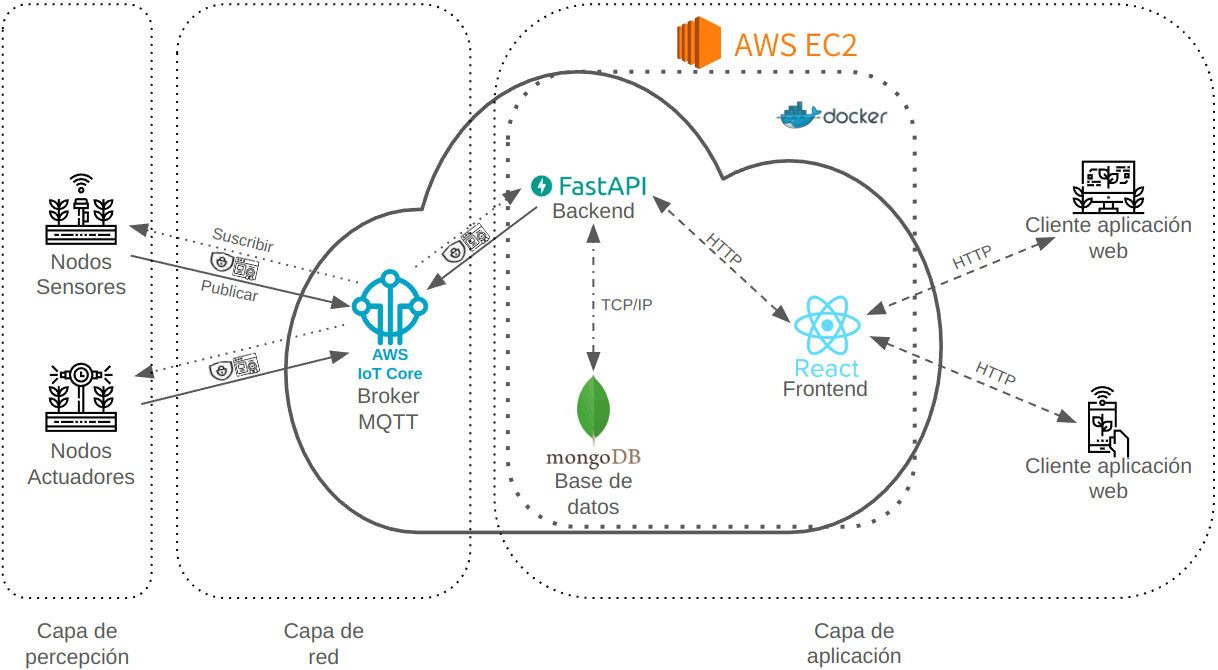
\includegraphics[width=.99\textwidth]{./Images/14.png}
    \caption{Arquitectura de la solución propuesta.}
    \label{fig:arquitectura}
\end{figure}

La arquitectura planteada para el desarrollo del trabajo sigue el modelo de
tres capas típico de un sistema IoT: percepción, red y aplicación.

\subsection{Capa de percepción}

La capa de percepción está constituida por los nodos sensores y actuadores, que
se encargan de recopilar datos del entorno y ejecutar acciones específicas en
función de los parámetros configurados.

Cada nodo sensor incluye un microcontrolador ESP-WROOM-32, este se conecta a
diversos sensores que miden parámetros como temperatura ambiente, humedad
relativa, presión atmosférica, luminosidad, concentración de $CO_2$, pH,
conductividad eléctrica, temperatura de la solución nutritiva, nivel de
líquidos, consumo eléctrico, entre otros. Los nodos actuadores, por su parte,
cuentan con relés para controlar dispositivos como ventiladores, iluminación y
sistemas de recirculación de nutrientes.

Los nodos están conectados a una red Wi-Fi local, lo que les permite establecer
comunicación con la red y transmitir los datos de los sensores hacia el
servidor IoT. La transmisión de datos se realiza con el protocolo MQTT.

\subsection{Capa de red}

La capa de red está compuesta por la infraestructura que gestiona la
comunicación entre los nodos sensores y actuadores y la plataforma de backend.
Los nodos sensores y actuadores se conectan a la red Wi-Fi local, lo que les
permite acceder a internet y a la infraestructura de la nube. Una vez
conectados, los dispositivos transmiten los datos a través del protocolo MQTT.

La comunicación entre los nodos y el broker MQTT se asegura mediante el uso de
certificados de seguridad, los que garantizan la autenticación de los
dispositivos y el cifrado de los datos.

El broker MQTT utilizado en este trabajo es AWS IoT Core, un servicio
completamente gestionado que permite establecer una conexión segura y escalable
entre los dispositivos IoT y la nube. Este broker actúa como intermediario para
la transmisión de datos entre los nodos y la capa de aplicación.

\subsection{Capa de aplicación}

La capa de aplicación es responsable del procesamiento, almacenamiento y
visualización de los datos recopilados por los nodos. Para esta capa, se
implementó el servidor IoT en la nube utilizando el servicio \textit{AWS EC2},
que permite ejecutar aplicaciones y servicios en instancias virtuales.

El procesamiento y la gestión de datos se realiza a través de un backend
desarrollado con FastAPI, mientras que la base de datos MongoDB se utiliza para
el almacenamiento de la información. Además, se implementó una interfaz gráfica
de usuario en React para la visualización y gestión de los datos. Todos estos
servicios fueron desplegados a través de contenedores Docker.

%----------------------------------------------------------------------------------------
%	SECTION 2
%----------------------------------------------------------------------------------------
\section{Modelo de datos}

En esta sección se presenta el modelo de datos implementado en el sistema.

La figura \ref{fig:modelo de datos} permite visualizar las principales
colecciones y sus relaciones dentro de la base de datos. El diseño del modelo
de datos se desarrolló en base a los tipos de datos proporcionados por los
sensores, así como los requerimientos técnicos establecidos para el sistema.

\begin{figure}[H]
    \centering
    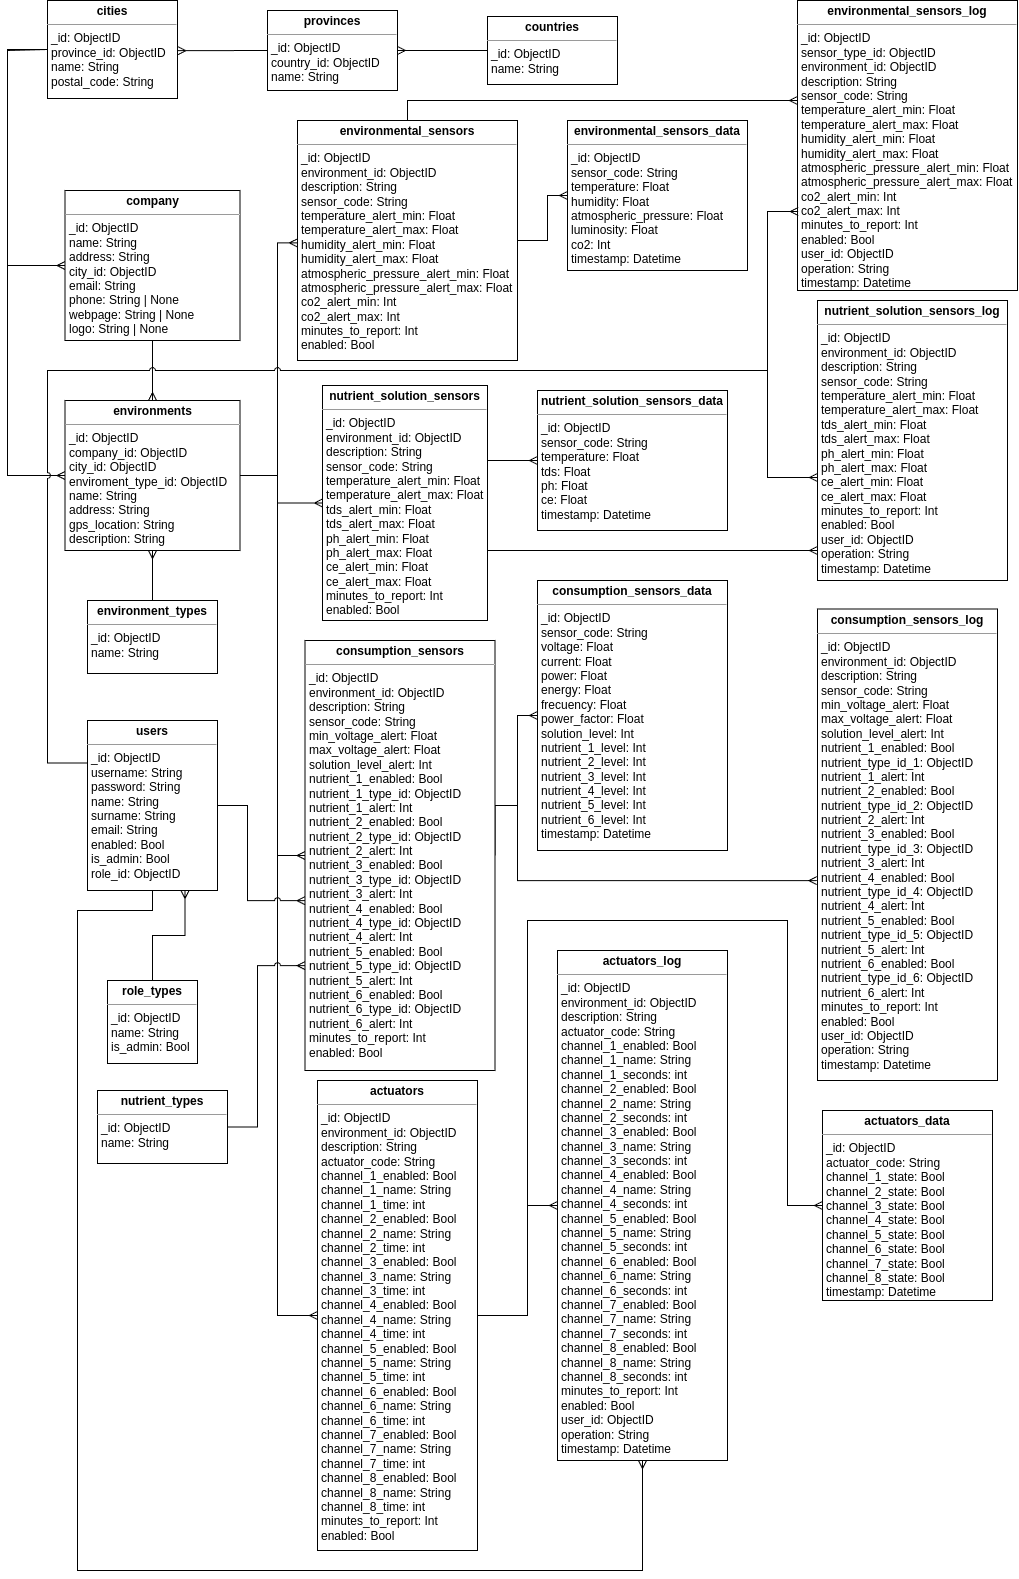
\includegraphics[width=.99\textwidth]{./Images/15.png}
    \caption{Modelo de datos implementado.}
    \label{fig:modelo de datos}
\end{figure}

El modelo de datos se estructuró en colecciones dentro de MongoDB, organizadas
en las siguientes categorías principales:

\subsection{Parametrización del sistema}

\begin{itemize}
    \item Colecciones de configuración básica: países, provincias, ciudades, empresa.
    \item Colecciones para gestión de espacios: ambientes y tipos de ambientes.
    \item Colecciones específicas del dominio: tipos de nutrientes.
\end{itemize}

\subsection{Gestión de usuarios y roles}

\begin{itemize}
    \item Colección de usuarios y roles: almacena información de los usuarios y sus
          credenciales.
    \item Colección de roles: se plantea como funcionalidad futura, para poder
          parametrizar permisos para cada tipo de rol.
\end{itemize}

\subsection{Sensores y actuadores}
\begin{itemize}
    \item Colecciones de sensores y actuadores: almacena la información de cada tipo de
          dispositivo, los parámetros de alerta y la frecuencia de muestreo.
    \item Colecciones de datos históricos: registran las mediciones vinculadas a cada
          dispositivo mediante identificadores únicos.
\end{itemize}

\subsection{Auditoría y seguimiento}
\begin{itemize}
    \item Colecciones de logs: permiten registrar los cambios en las configuraciones de
          sensores y actuadores realizados por los usuarios.
\end{itemize}

El modelo de datos completo del sistema, puede consultarse en el apéndice
\ref{AppendixA}.

%----------------------------------------------------------------------------------------
%	SECTION 3
%----------------------------------------------------------------------------------------
\section{Servidor IoT}

En esta sección se presenta la arquitectura del sistema y se detallan las
tecnologías utilizadas y la arquitectura del servidor.

\subsection{Arquitectura del servidor}

La arquitectura del servidor está compuesta por tres componentes principales:
backend, capa de datos y frontend, como se muestra en la figura
\ref{fig:arquitectura servidor}.

\begin{figure}[H]
    \centering
    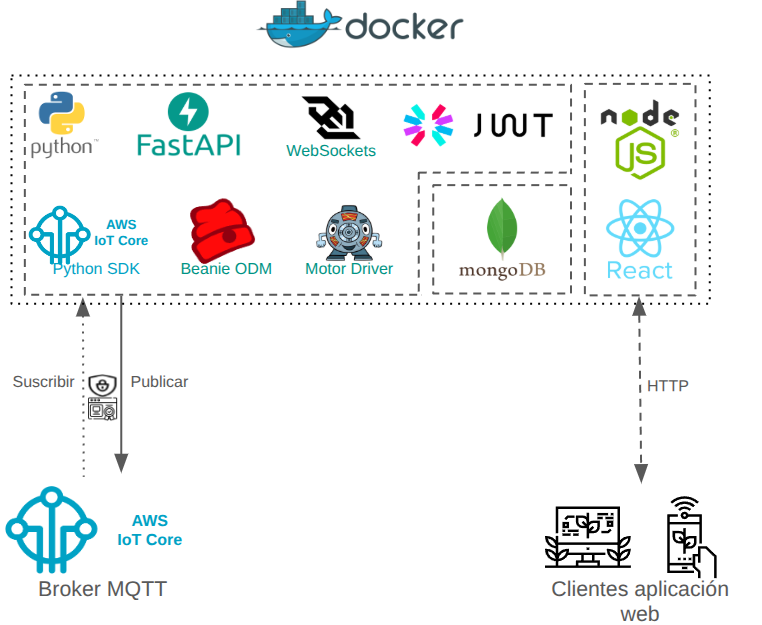
\includegraphics[width=.97\textwidth]{./Images/16.png}
    \caption{Arquitectura del servidor del sistema IoT.}
    \label{fig:arquitectura servidor}
\end{figure}

A continuación, se describe brevemente cada uno de estos componentes:

\begin{itemize}
    \item Backend: implementado con FastAPI, expone una API REST que permite gestionar
          sensores, actuadores, ambientes y usuarios. Incluye autenticación y
          autorización basada en JWT, integración con MongoDB a través de Beanie
          \cite{BeaniODM} y Motor \cite{MotorMongoDB}, conexión con el broker MQTT para
          la comunicación con los dispositivos IoT implementada con el SDK (del inglés,
          \textit{Software Development Kit}) de AWS IoT para Python \cite{AWSIoTSDK} y
          soporte para comunicaciones en tiempo real con clientes mediante WebSocket
          \cite{FastAPIWebSockets}.

    \item Capa de datos: utiliza MongoDB como base de datos NoSQL. La información se
          organiza en colecciones que almacenan datos de sensores, actuadores, usuarios,
          ambientes y registros de configuración.

    \item Frontend: desarrollado en React, permite a los usuarios visualizar datos en
          tiempo real y configurar el sistema. Se conecta con la API REST del backend y
          utiliza WebSocket \cite{SocketIO} para actualizaciones en tiempo real.
\end{itemize}

%----------------------------------------------------------------------------------------
%	SECTION 4
%----------------------------------------------------------------------------------------
\section{Desarrollo del backend}

En esta sección se detallan los aspectos clave en el diseño y desarrollo del
servidor backend, así como la lógica de negocio implementada.

\subsection{Diseño de la API}

El diseño se estructuró en base a las necesidades del sistema y los
requerimientos funcionales y no funcionales establecidos. Se organizaron los
archivos en carpetas de acuerdo a su funcionalidad. % Se definieron los modelos
% de datos utilizando la librería Beanie y se implementaron los endpoints para
% realizar las operaciones necesarias en la API.

La tabla \ref{tab:endpoints} presenta un resumen de los principales endpoints
de la API, junto con una breve descripción de la acción y el método HTTP
utilizado.

\begin{table}[H]
    \centering
    \caption[Resumen de principales endpoints de la API]{Resumen de principales endpoints de la API.}
    \begin{tabular}{l l l}
        % \begin{tabular}{p{1.3cm}p{5.7cm}p{4.9cm}}
        \toprule
        \textbf{Método} & \textbf{Endpoint}                 & \textbf{Acción}            \\
        \midrule
        GET             & /mqtt/test                        & Test conexión cliente MQTT \\
        POST            & /mqtt/publish                     & Publicar en tópico MQTT    \\
        \midrule
        POST            & /login                            & Login de usuarios          \\
        GET             & /renew-token                      & Renovar token              \\
        \midrule
        GET             & /users/                           & Obtener usuarios           \\
        \midrule
        GET             & /environments/                    & Obtener ambientes          \\
        \midrule
        GET             & /actuators/                       & Obtener actuadores         \\
        \midrule
        GET             & /sensors/environmental/           & Obtener sensores           \\
        \midrule
        GET             & /sensors/nutrients/solution/      & Obtener sensores           \\
        \midrule
        GET             & /sensors/consumption/             & Obtener sensores           \\
        \midrule
        GET             & /actuators/data/                  & Obtener datos históricos   \\
        GET             & /sensors/environmental/data/      & Obtener datos históricos   \\
        GET             & /sensors/consumption/data/        & Obtener datos históricos   \\
        GET             & /sensors/nutrients/solution/data/ & Obtener datos históricos   \\
        \bottomrule
        \hline
    \end{tabular}
    \label{tab:endpoints}
\end{table}

El listado completo de endpoints de la API se puede consultar en el apéndice
\ref{AppendixB}.

\subsection{Autenticación y autorización}

Se implementó un sistema de autenticación basado en JWT, que permite a los
usuarios acceder a la API de manera segura. La autenticación se realiza
mediante el envío de las credenciales del usuario en el cuerpo de la solicitud,
y el servidor responde con un token JWT que se utiliza para autenticar las
solicitudes posteriores.

El token JWT contiene la información del usuario, este token se envía en el
encabezado de las solicitudes a la API. El servidor verifica la validez del
token y permite o deniega el acceso a los recursos solicitados. El token se
diseño para que tuviera vencimiento, por lo que se implementó un sistema de
renovación que permite a los usuarios mantener su sesión activa sin necesidad
de autenticarse nuevamente con sus credenciales.

El código de la implementación de la autenticación y autorización se puede
consultar en el apéndice \ref{AppendixC}.

La figura \ref{fig:esquema autenticacion} muestra el esquema de autenticación,
autorización y renovación de tokens implementado en el sistema.

\begin{figure}[H]
    \centering
    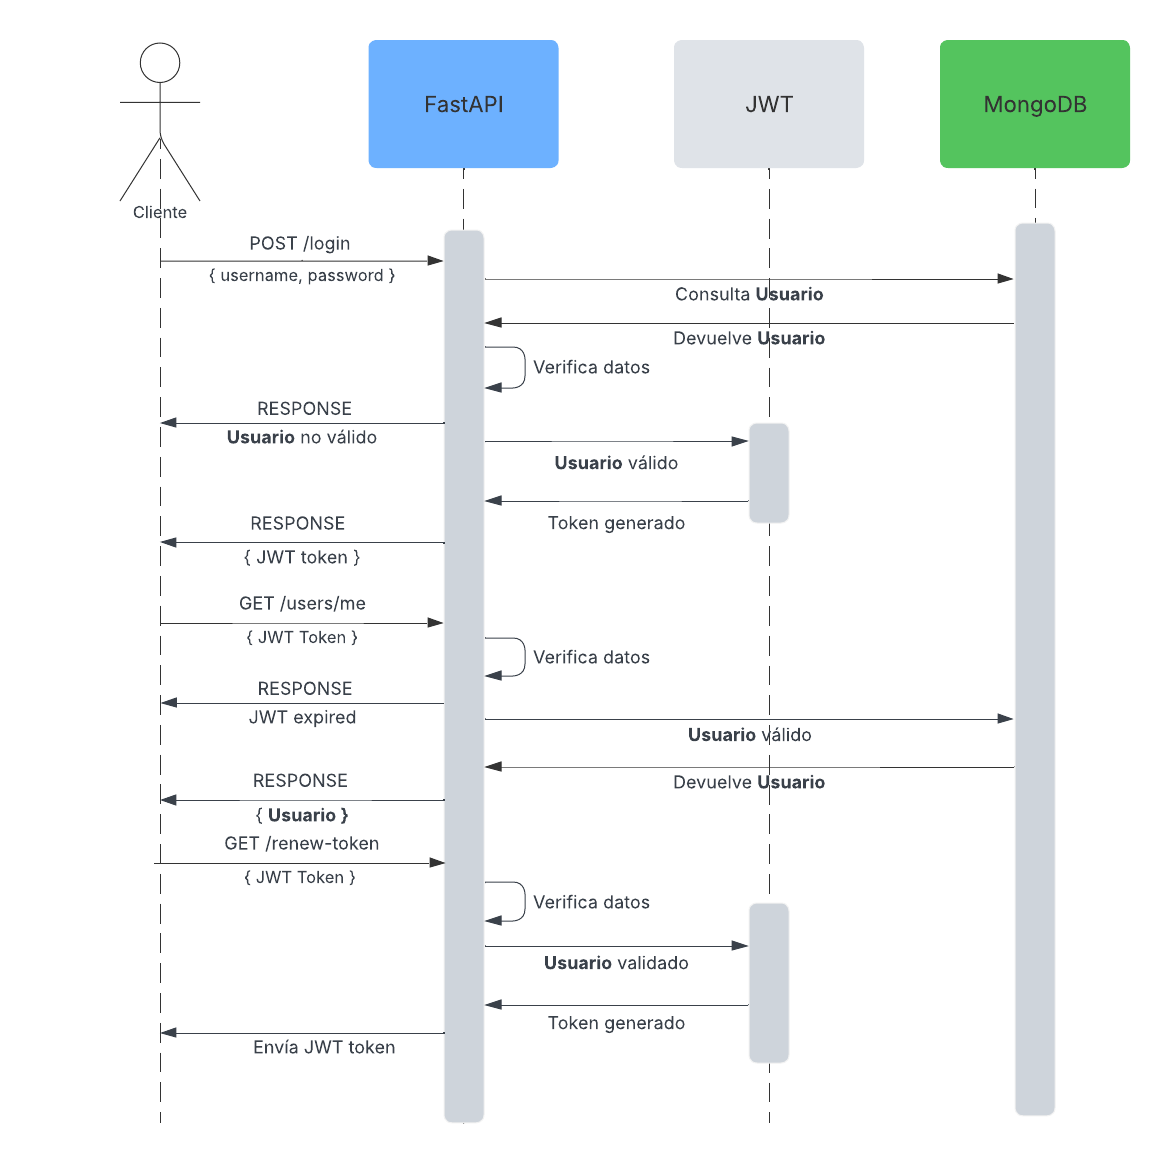
\includegraphics[width=.78\textwidth]{./Images/17.png}
    \caption{Esquema de autenticación y autorización.}
    \label{fig:esquema autenticacion}
\end{figure}

\subsection{Persistencia de datos}

En FastAPI, cada modelo representa una colección en la base de datos e incluye
los campos necesarios para almacenar la información requerida. La comunicación
entre el backend y la base de datos se realizó a través de la biblioteca Motor,
que proporciona una interfaz asíncrona para interactuar con MongoDB. Además se
utilizó el ODM (del inglés, \textit{Object Document Mapper}), a través de la
biblioteca Beanie, que permite definir modelos y realizar consultas y
operaciones sobre la base de datos de manera sencilla.

La figura \ref{fig:diagrama de clases} muestra un ejemplo de la relación entre
los modelos implementados en el sistema y los métodos HTTP de la colección
\texttt{EnvironmentalSensor}.

\begin{figure}[H]
    \centering
    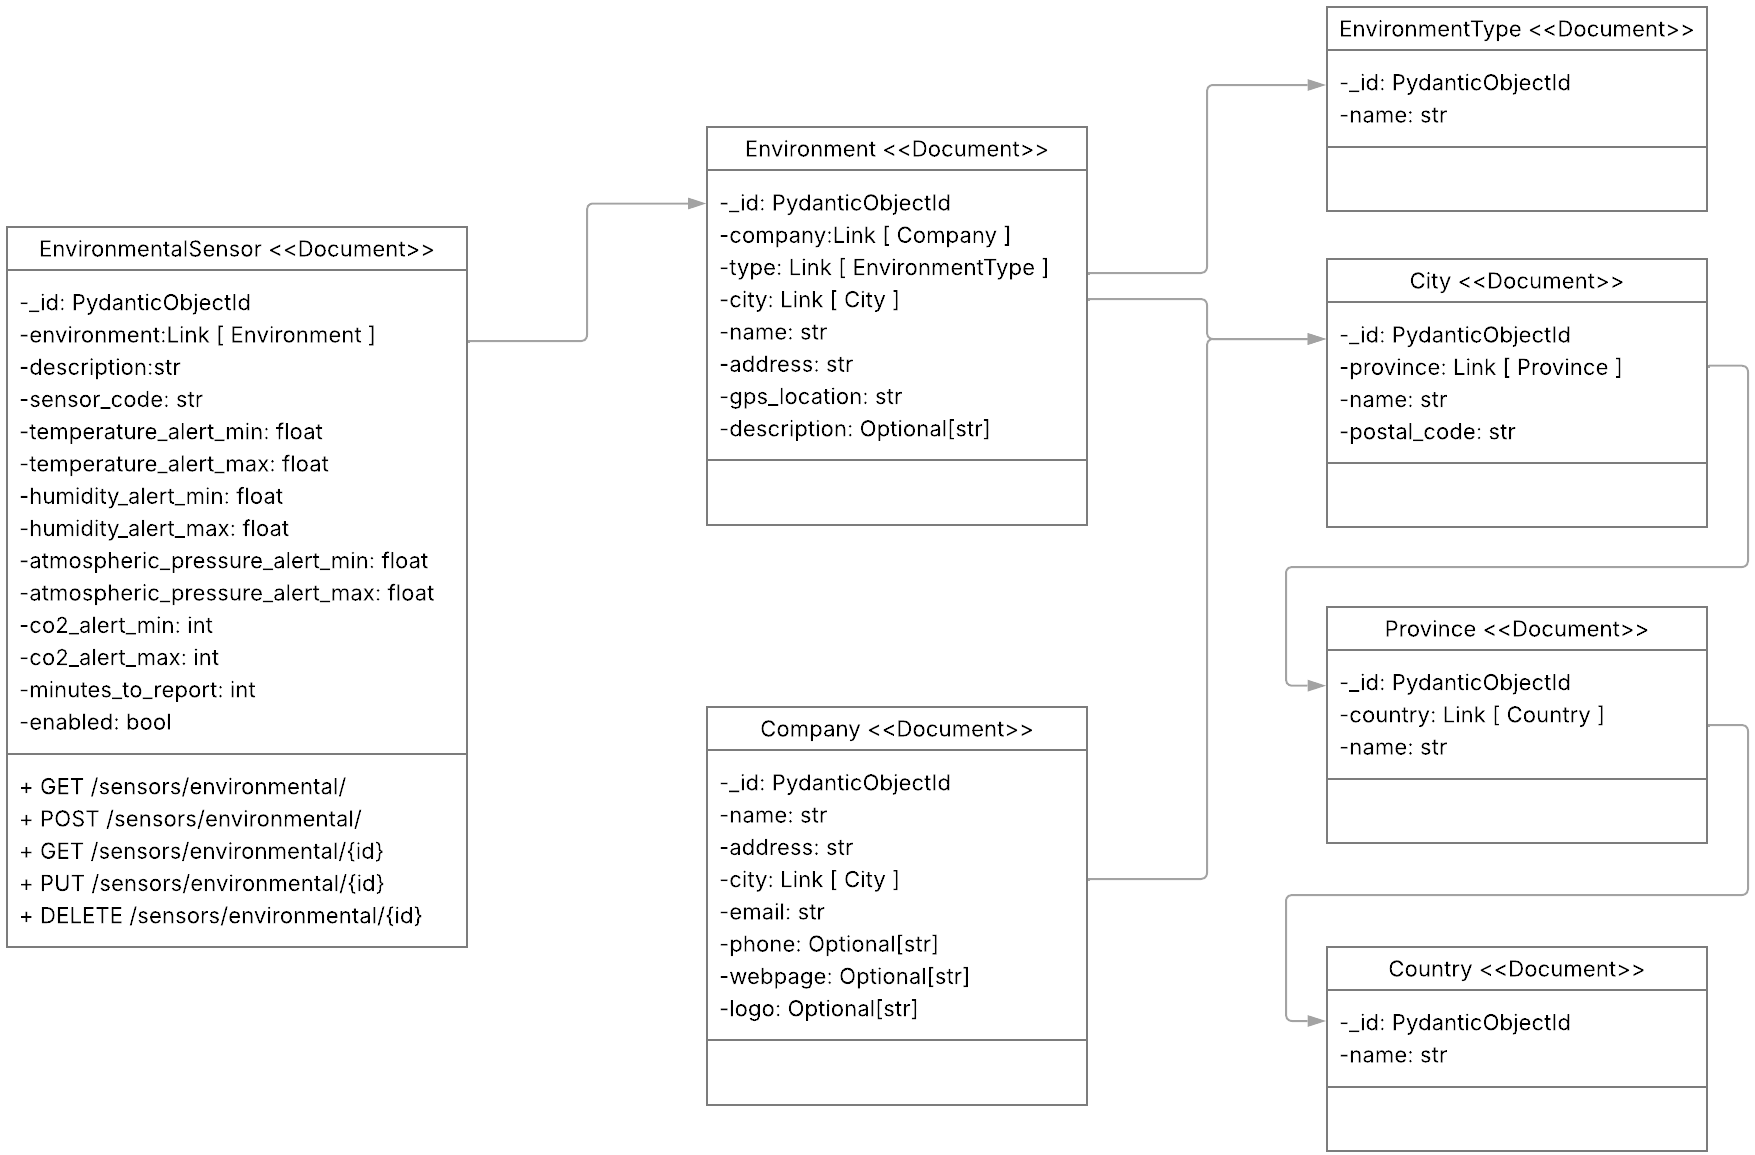
\includegraphics[width=.85\textwidth]{./Images/18.png}
    \caption{Diagrama de clases de los modelos implementados.}
    \label{fig:diagrama de clases}
\end{figure}

Como se mencionó anteriormente, los datos se almacenan en MongoDB. Para
establecer la conexión con la base de datos, se utiliza el cliente asíncrono de
la biblioteca Motor, mientras que la inicialización de los modelos se realiza
% mediante la función \texttt{init\_beanie}. Esta función configura los modelos y
mediante la función \texttt{init\_beanie} del ODM Beanie. Esta función
configura los modelos y establece la conexión con la base de datos. En la
cadena de conexión se especifica el nombre de usuario, la contraseña y la
dirección del servidor de MongoDB.

La figura \ref{fig:conexion mongo} ilustra los pasos necesarios para establecer
la conexión entre FastAPI y MongoDB.

\begin{figure}[H]
    \centering
    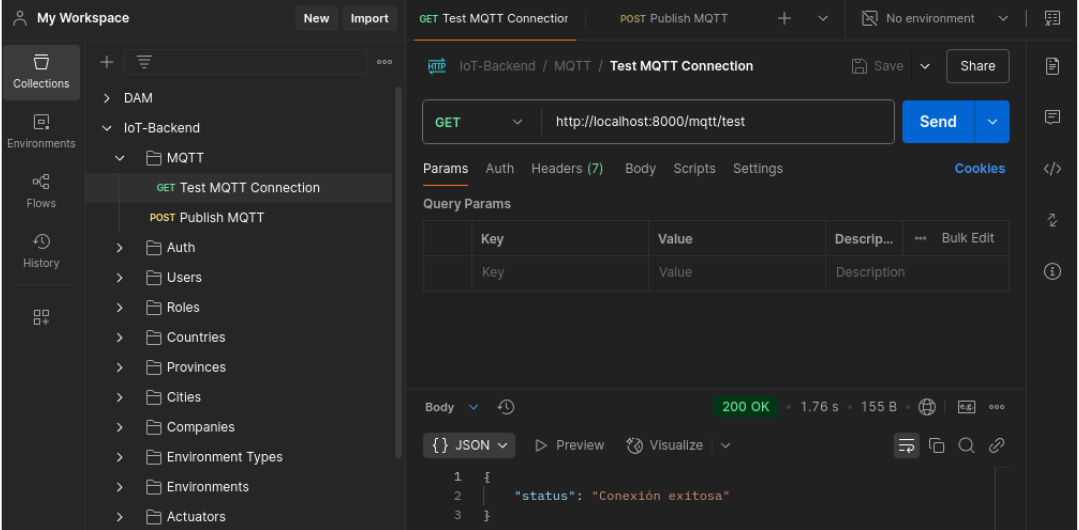
\includegraphics[width=.85\textwidth]{./Images/19.png}
    \caption{Pasos para la conexión de FastAPI y MongoDB.}
    \label{fig:conexion mongo}
\end{figure}

El código para establecer la conexión y la inicialización de los modelos se
puede consultar en el apéndice \ref{AppendixD}.

\subsection{Comunicación con el broker MQTT}

A continuación, se describe la implementación de la comunicación con el broker
MQTT.

\subsubsection{Pasos en AWS IoT Core}

Este apartado detalla los pasos realizados en AWS IoT Core para crear y
configurar el objeto \textit{Thing} y los certificados de seguridad necesarios
para establecer la conexión con el broker MQTT.

\begin{enumerate}
    \item Se creó un objeto \textit{Thing} en AWS IoT Core, que representa un dispositivo
          IoT. Este objeto se utiliza para gestionar la conexión y la comunicación con el
          broker.
    \item Se generaron certificados de seguridad y claves privadas para el objeto
          \textit{Thing}, y se descargó el certificado raíz de Amazon. Estos elementos
          son necesarios para autenticar la conexión, garantizar el cifrado de los datos
          transmitidos y establecer una comunicación segura con el broker MQTT.
    \item Se definieron las políticas de acceso necesarias para el objeto \textit{Thing},
          a fin de permitir publicar y suscribirse a los tópicos correspondientes.
\end{enumerate}

\textbf{Políticas de acceso:} determinan los permisos del cliente para publicar,
suscribirse y recibir mensajes en los tópicos. Se aplican a los certificados
generados para el cliente y controlan el acceso a los recursos de AWS IoT Core.

Definidas en formato JSON, estas políticas garantizan que solo los clientes
autorizados puedan interactuar con los recursos y operar en los tópicos
correspondientes. Además, pueden configurarse de manera específica para cada
\textit{Thing}, lo que permite ejercer un control granular sobre los permisos
de acceso.

En el Apéndice \ref{AppendixE} se puede visualizar un ejemplo de política de
acceso definida para el objeto \textit{Thing}.

\subsubsection{Implementación de MQTT en FastAPI}
Una vez que se creó y se configuró el objeto \textit{Thing} en AWS IoT Core, se
procedió a la implementación de la conexión del broker con FastAPI. Para ello,
se utilizó la SDK de AWS IoT para Python, que proporciona una interfaz sencilla
para conectarse al broker y gestionar la comunicación con los dispositivos IoT.

Se implementó un cliente MQTT que se conecta al broker con los certificados
generados previamente. Este cliente permite publicar y suscribirse a los
tópicos correspondientes, lo que facilitó la comunicación entre el servidor y
los dispositivos IoT.

En la aplicación FastAPI se definieron dos rutas claves para la chequear la
comunicación con AWS IoT Core:

\begin{enumerate}
    \item Una ruta para verificar la conexión con el broker MQTT.
    \item Una ruta para enviar mensajes a un tópico y comprobar la comunicación entre el
          servidor y el broker.
\end{enumerate}

La figura \ref{fig:test_mqtt} muestra los pasos realizados para verificar la
conexión con el broker MQTT.

\begin{figure}[H]
    \centering
    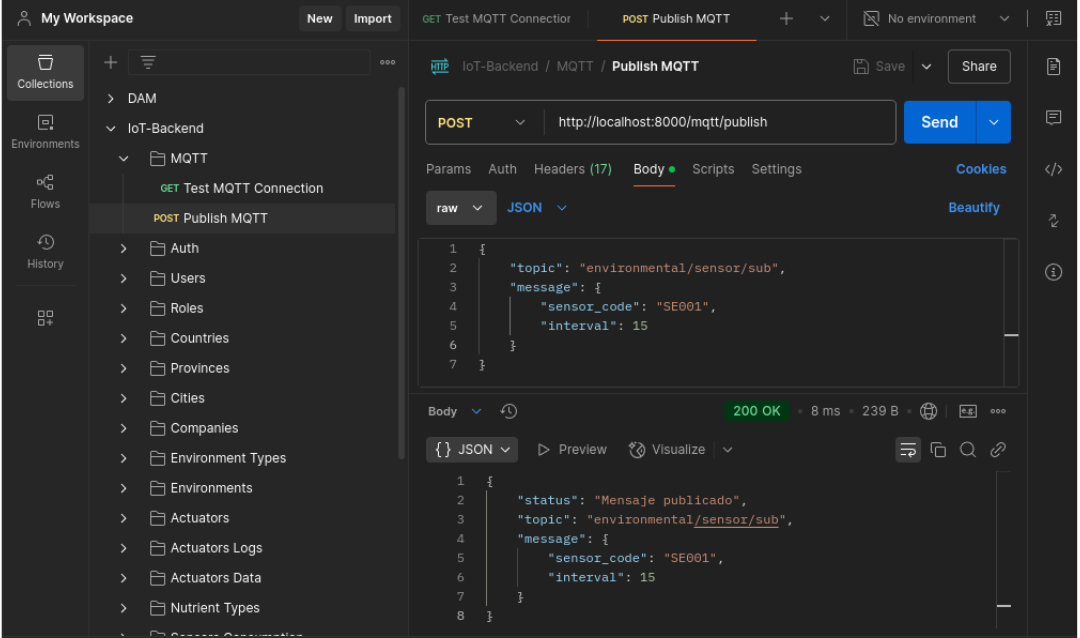
\includegraphics[width=.90\textwidth]{./Images/20.png}
    \caption{Pasos para verificar la conexión con el broker MQTT.}
    \label{fig:test_mqtt}
\end{figure}

La figura \ref{fig:publish_mqtt} muestra los pasos realizados para publicar un
mensaje en un tópico específico.

\begin{figure}[H]
    \centering
    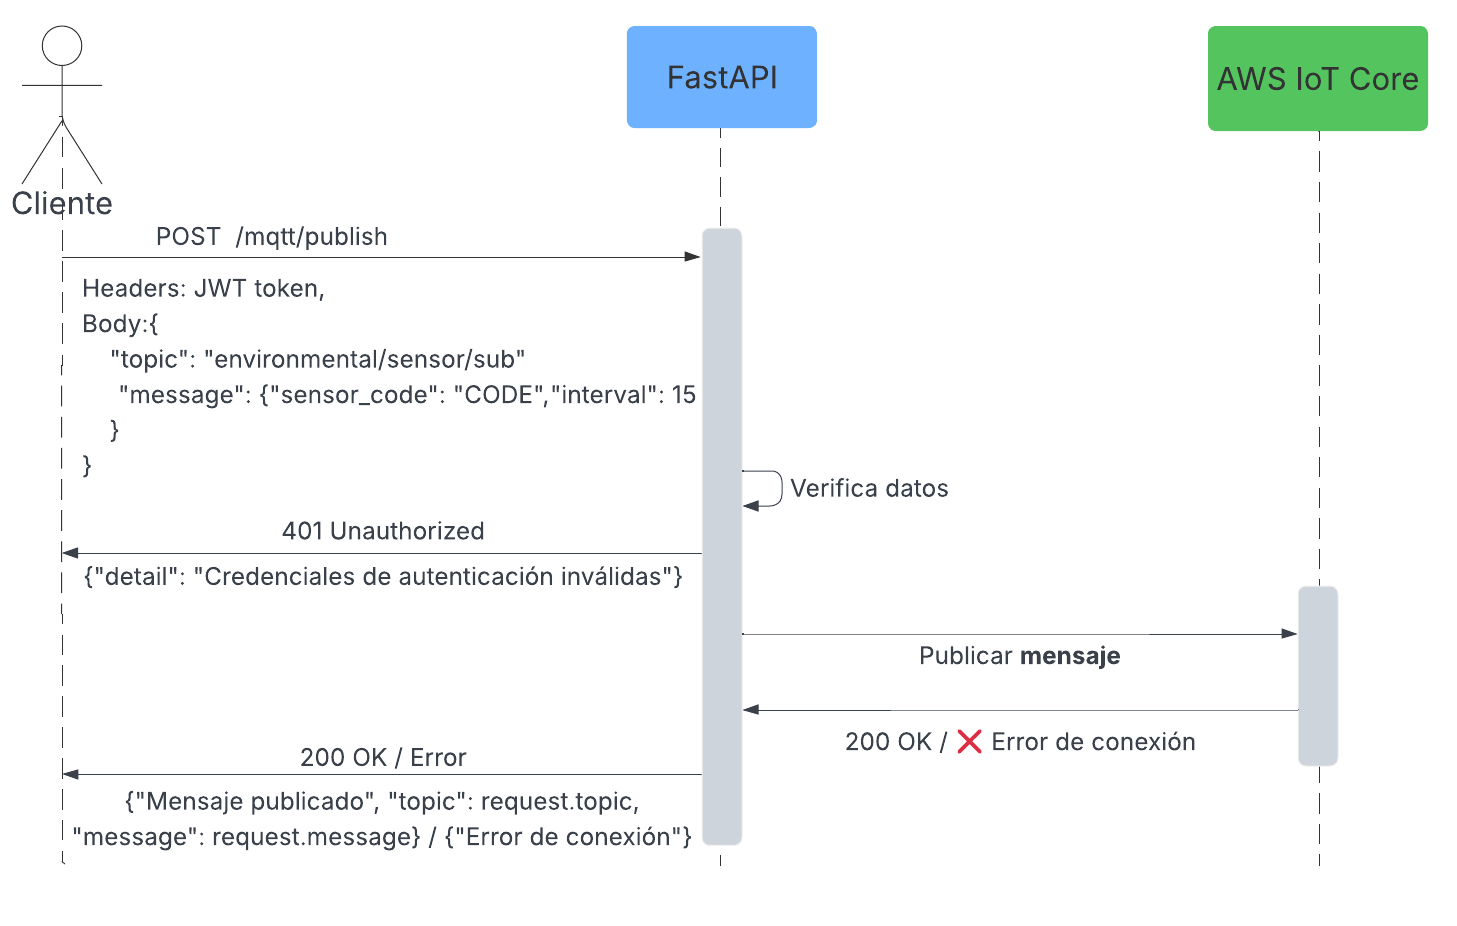
\includegraphics[width=.90\textwidth]{./Images/21.png}
    \caption{Pasos para publicar un mensaje en un tópico específico.}
    \label{fig:publish_mqtt}
\end{figure}

\subsubsection{Comunicación con MQTT en FastAPI}

Además de las rutas anteriores, en FastAPI se implementaron métodos para
suscribirse a los tópicos, recibir mensajes de los nodos y publicar en los
tópicos correspondientes.

Al iniciarse el servidor, el cliente MQTT establece la conexión con el broker y
se suscribe a los tópicos definidos. Los mensajes recibidos son procesados,
almacenados en MongoDB y enviados al frontend mediante WebSocket, lo que
permite actualizar la interfaz en tiempo real. Este cliente, que maneja la
conexión, publicación y suscripción, se inicializa junto con FastAPI para
asegurar una comunicación eficiente.

La figura \ref{fig:cliente_mqtt} muestra los pasos de cómo la aplicación
FastAPI se conecta al broker MQTT y se suscribe a los tópicos solicitados.

\begin{figure}[H]
    \centering
    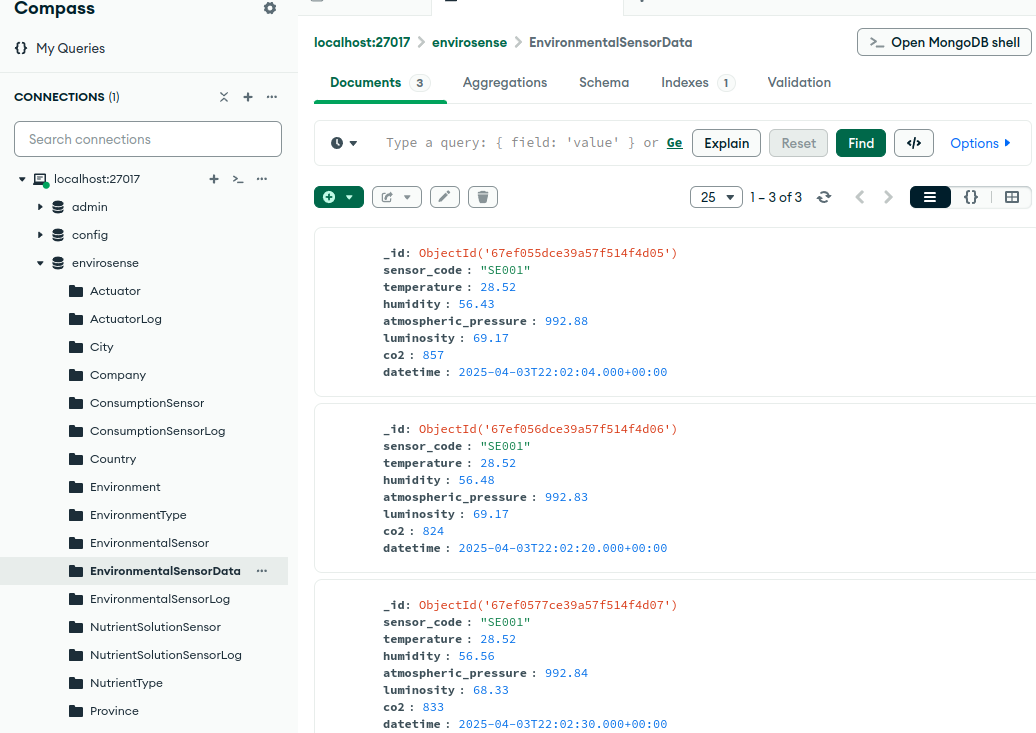
\includegraphics[width=.75\textwidth]{./Images/22.png}
    \caption{Pasos para la conexión del cliente MQTT.}
    \label{fig:cliente_mqtt}
\end{figure}

El código completo de la implementación de la conexión con el broker MQTT se
encuentra en el Apéndice \ref{AppendixE}.

\subsection{Implementación de WebSockets}

La comunicación en tiempo real se implementó mediante el módulo
\texttt{websockets} de FastAPI, con una ruta específica para que los clientes
se conecten y reciban datos actualizados de sensores y actuadores. La conexión
permanece activa mientras sea válida, y se cierra en caso de error o falta de
autorización.

El cliente debe enviar un token válido por \texttt{Authorization} o
\texttt{Query Params}. Si es válido, el servidor acepta la conexión y la
gestiona a través de la clase \texttt{WebSocketManager}.

Esta clase administra las conexiones activas, clientes y el envío de datos en
tiempo real. Además, mantiene un caché con los últimos valores por tipo de
sensor para optimizar el rendimiento. Al recibir nuevos datos, el servidor
actualiza el caché y los transmite a todos los clientes conectados.

El código de la implementación se encuentra en el apéndice \ref{AppendixF}, y
la figura \ref{fig:websocket} ilustra el proceso de conexión.

\begin{figure}[H]
    \centering
    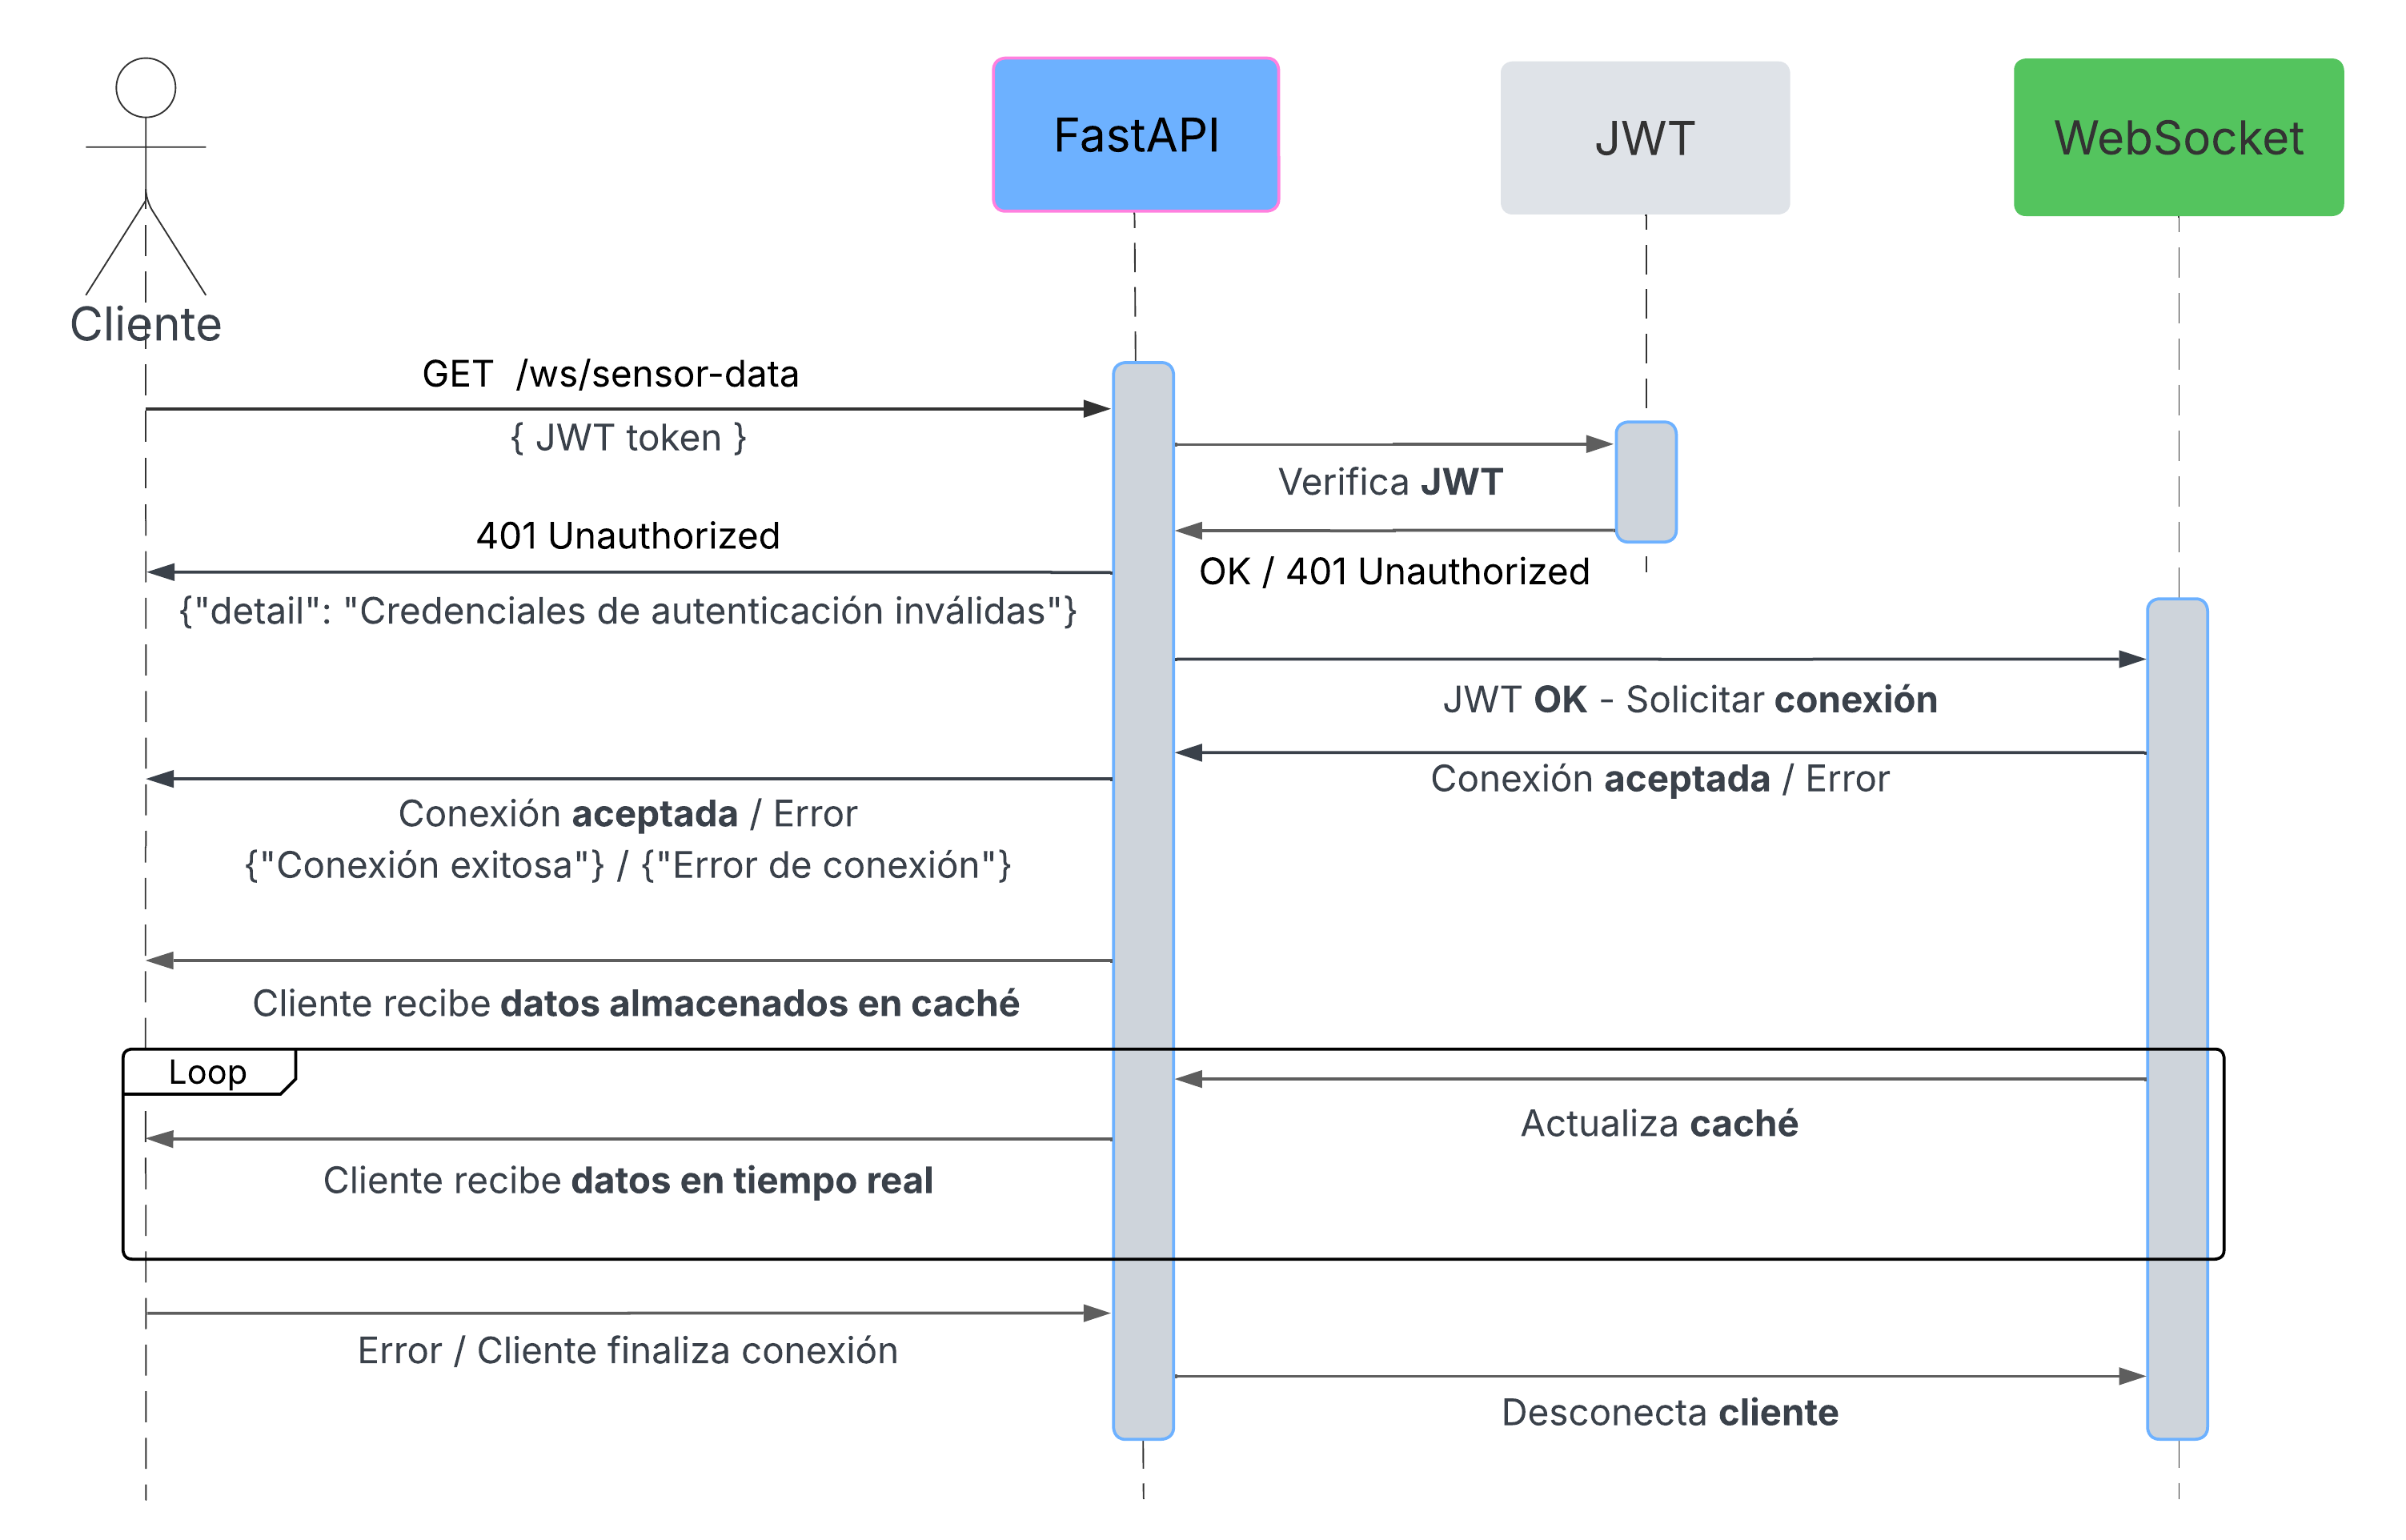
\includegraphics[width=.90\textwidth]{./Images/23.png}
    \caption{Pasos para establecer la conexión WebSocket.}
    \label{fig:websocket}
\end{figure}

%----------------------------------------------------------------------------------------
%	SECTION 5
%----------------------------------------------------------------------------------------
\section{Desarrollo del frontend}

En esta sección se describe el diseño y desarrollo de la interfaz de usuario,
enfocada en la visualización de datos en tiempo real y la gestión de
dispositivos a través de una aplicación web.

\subsection{Tecnologías utilizadas}

El frontend se desarrolló a través de la biblioteca \texttt{React}
\cite{React}. Para los estilos y la disposición visual se utilizó la biblioteca
\texttt{React Bootstrap} \cite{ReactBootstrap}. %, una biblioteca de componentes de interfaz de
%usuario basada en Bootstrap, que permite crear aplicaciones web responsivas y
%modernas de manera sencilla. 
Para los iconos de la interfaz se utilizó \texttt{Bootstrap Icons}
\cite{BootstrapIcons}, que proporciona una amplia variedad de iconos gratuitos
personalizables y fáciles de usar.

La comunicación con el servidor se implementó mediante la biblioteca
\texttt{axios} \cite{Axios} para realizar solicitudes HTTP, mientras que la
recepción de datos en tiempo real se logró con la implementación de un
\texttt{WebSocket} nativo, a través de un \texttt{hook} personalizado
desarrollado en React.

La gestión del estado de autenticación y control de sesiones se implementó con
\texttt{Redux Toolkit} \cite{ReduxToolkit} y la navegación entre páginas se
gestionó a través de la biblioteca \texttt{react-router-dom}
\cite{ReactRouter}.

Para la visualización de los gráficos, se empleó la librería \texttt{Recharts}
\cite{Recharts}, mientras que para la representación de tablas se utilizó la
biblioteca \texttt{React Data Table Component} \cite{ReactDataTable}.

\subsection{Arquitectura de la interfaz}

La aplicación se estructuró en torno a un componente principal de
\texttt{Layout}, que organiza la navegación mediante un \texttt{sidebar}
lateral y un \texttt{navbar} superior.

Cada sección de la interfaz de usuario corresponde a un módulo de funcionalidad
específica (como visualización en tiempo real, reportes, configuración de
ambientes y dispositivos, parámetros y administración de usuarios), que son
renderizados dinámicamente en función de la ruta activa.

% La aplicación se estructuró en torno a un componente principal de
% \texttt{Layout}, que organiza la navegación mediante un \texttt{sidebar}
% lateral y una \texttt{navbar} superior.

% La aplicación implementa un sistema de navegación basado en rutas mediante la
% biblioteca de enrutamiento \texttt{react-router-dom} \cite{ReactRouter}, donde
% cada módulo funcional se estructura como un componente independiente, lo que
% permite un fácil mantenimiento y escalabilidad. La estructura de carpetas se
% organizó en función de los módulos y componentes, facilitando la localización y
% modificación de los mismos.

\subsection{Componentes principales de la interfaz de usuario}

A continuación, se presenta un detalle de los principales componentes
desarrollados para la construcción de la interfaz:

\subsubsection{Gestión de autenticación}

La autenticación se implementó mediante un \texttt{hook} denominado
\texttt{useAuthStore}, basado en \texttt{Redux Toolkit}. Este módulo gestiona
el inicio de sesión, la validación del token y el cierre de sesión de los
usuarios, para asegurar el acceso restringido a las funcionalidades de la
plataforma.

Al iniciar sesión, se almacena el token en el \texttt{localStorage} del
navegador, lo que permite mantener la sesión activa y acceder a las
funcionalidades de la aplicación. El token se envía en cada solicitud a la API
para autenticar al usuario y garantizar la seguridad de la comunicación.

La figura \ref{fig:login} muestra la pantalla de inicio de sesión, donde los
usuarios ingresan sus credenciales para acceder a la aplicación web.

\begin{figure}[H]
    \centering
    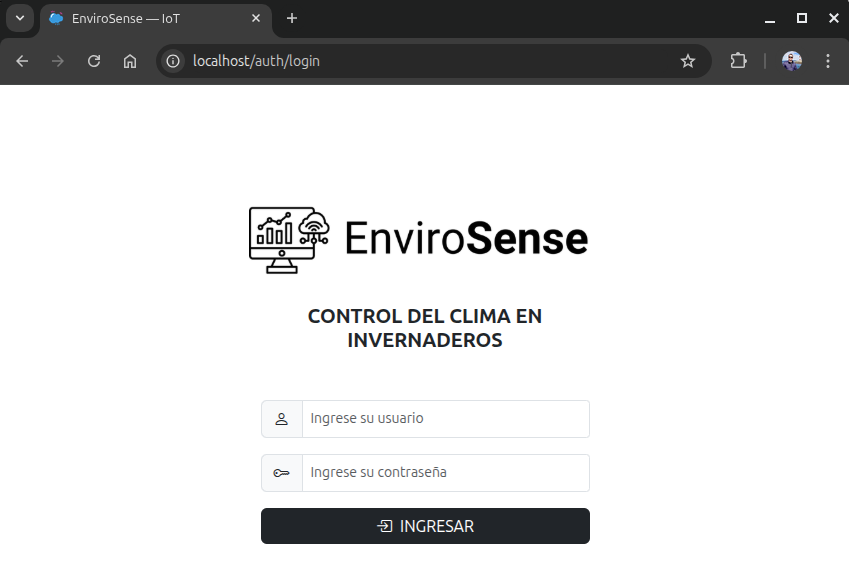
\includegraphics[width=0.65\textwidth]{./Images/24_login.png}
    \caption{Pantalla de Login}
    \label{fig:login}
\end{figure}

\subsubsection{Layout}

El componente \texttt{Layout} organiza la estructura general de la aplicación e
incluye:
\begin{itemize}
    \item \textbf{SidebarComponent}: componente que muestra el menú lateral, con
          opciones de navegación entre los distintos módulos.
    \item \textbf{NavbarComponent}: barra superior que permite colapsar o expandir
          el menú lateral y contiene el botón de cierre de sesión.
\end{itemize}

La figura \ref{fig:layout} muestra la pantalla principal de la aplicación,
donde se puede observar la barra de navegación superior y el menú lateral desde
el rol \texttt{admin}.

\begin{figure}[H]
    \centering
    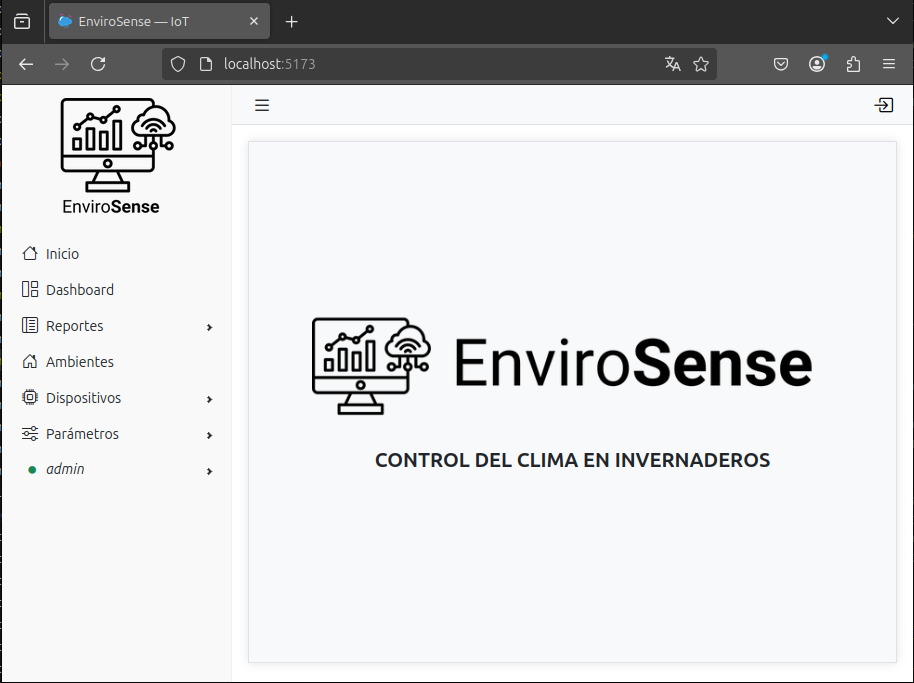
\includegraphics[width=0.75\textwidth]{./Images/25_layout.png}
    \caption{Estructura del componente Layout}
    \label{fig:layout}
\end{figure}

Además, esta pantalla permite visualizar los módulos disponibles en la
aplicación, como dashboard, reportes, ambientes, dispositivos, parámetros y
panel de usuario.

\subsubsection{Arquitectura de navegación y control de acceso}

La aplicación implementa un sistema de navegación que gestiona dinámicamente
las rutas públicas y privadas mediante la biblioteca \texttt{react-router-dom}.
Utiliza los componentes \texttt{Routes} para definir la estructura de
navegación y \texttt{Outlet} para renderizar sub-rutas.

Además, se implementa un flujo de acceso controlado por:

\begin{itemize}
    \item \textbf{Rutas públicas}: accesibles sin autenticación, como la página de
          inicio de sesión.
    \item \textbf{Rutas privadas}: requieren autenticación y autorización, como el
          acceso a los módulos de la aplicación.
    \item \textbf{Rutas restringidas}: accesibles solo para usuarios con los permisos
          adecuados, como reportes, la gestión de usuarios, ambientes, y dispositivos.
\end{itemize}

Este esquema asegura que los usuarios solo tengan acceso a las funcionalidades
correspondientes a sus permisos, como se ilustra en la figura
\ref{fig:navegacion}. Por ejemplo, un usuario \texttt{martin}, con permisos de
\texttt{usuario básico}, solo puede acceder al \texttt{Dashboard} y al panel de
usuario para consultar su información personal.

\begin{figure}[H]
    \centering
    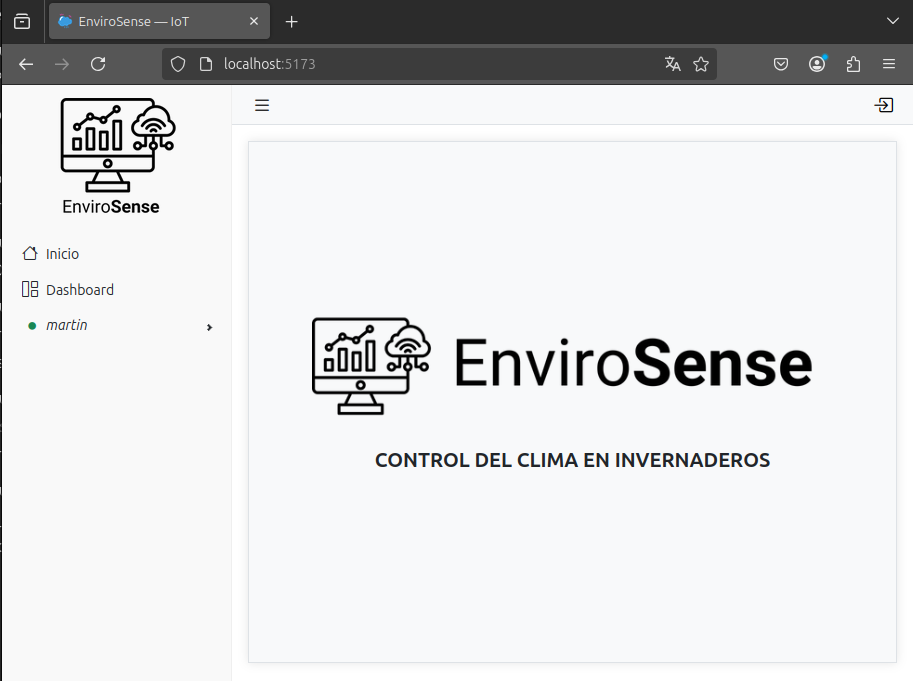
\includegraphics[width=0.75\textwidth]{./Images/26_navegacion.png}
    \caption{Sistema de navegación}
    \label{fig:navegacion}
\end{figure}

\subsection{Visualización de datos en tiempo real}

% Se desarrolló un \texttt{hook} personalizado llamado \texttt{useWebSocket}, el
% cual permite establecer conexiones WebSocket de forma sencilla. Este
% \texttt{hook} maneja los eventos de conexión, recepción de mensajes, cierre de
% conexión y manejo de errores, permitiendo recibir y procesar datos en tiempo
% real.

Se diseñó una página que muestra los datos de los actuadores y sensores de un
ambiente específico. Esta página permite visualizar los datos recopilados por
los sensores, así como el estado de los actuadores en tiempo real. Esta página
se actualiza automáticamente a medida que se reciben nuevos datos a través de
WebSocket.

La figura \ref{fig:dashboard} ilustra el \texttt{dashboard} de la aplicación,
donde se pueden observar los datos de los sensores y actuadores en tiempo real
de un ambiente específico.

\begin{figure}[H]
    \centering
    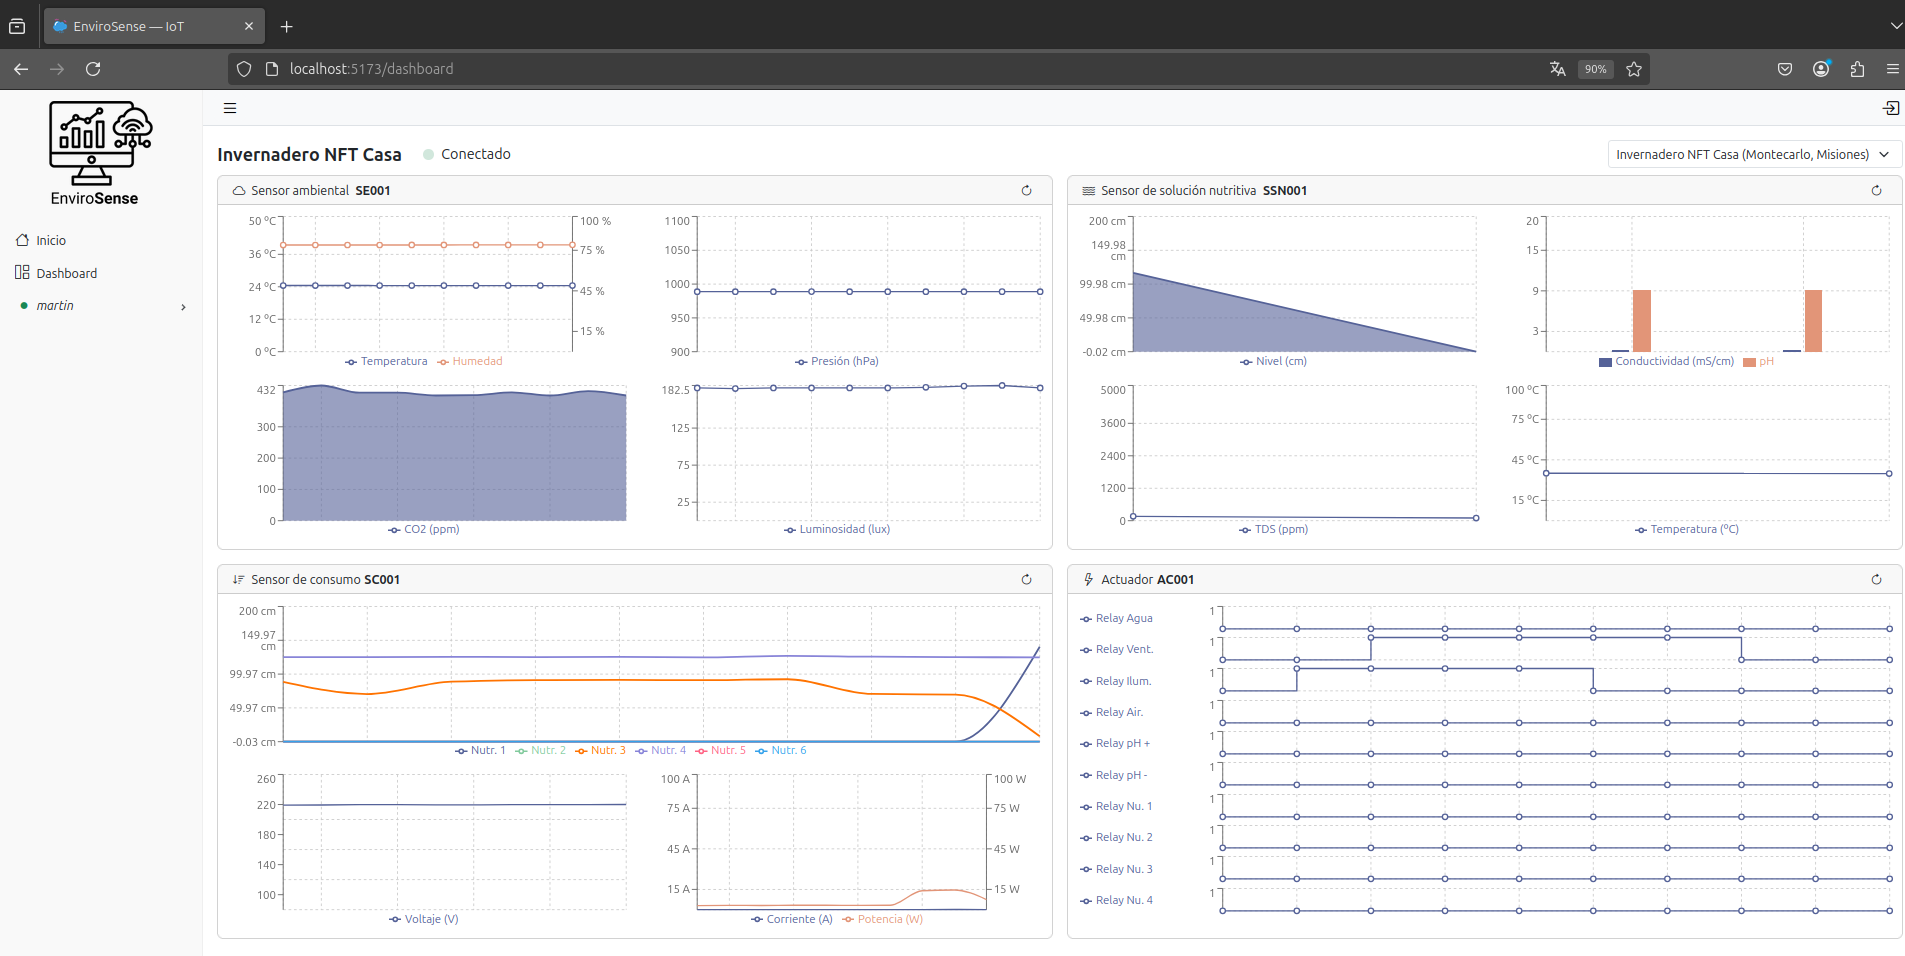
\includegraphics[width=0.99\textwidth]{./Images/27_dashboard.png}
    \caption{Visualización de datos en tiempo real}
    \label{fig:dashboard}
\end{figure}

\subsection{Reportes de datos históricos}

Se desarrollaron un conjunto de reportes que permiten visualizar los datos
históricos de los sensores y actuadores. % Estos reportes permiten realizar un análisis de
% los datos recopilados a lo largo del tiempo.
Los diferentes tipos de reportes están organizados en módulos independientes.

Cada reporte permite:
\begin{itemize}
    \item Filtrar los datos por dispositivo, rango de fechas y nivel de agregación
          temporal.
          \begin{itemize}
              \item \textbf{Actuadores:} el reporte permite visualizar la cantidad de veces que
                    se activó y el tiempo total de activación de cada canal del actuador en un
                    rango de fechas determinado.
              \item \textbf{Sensores:} el reporte permite visualizar el promedio de los datos
                    recopilados por cada sensor en un rango de fechas determinado.
          \end{itemize}
    \item Alternar entre una vista tabular y una vista gráfica.
    \item Consultar los datos procesados a través de la API del backend.
\end{itemize}

La figura \ref{fig:reportes_tabla_consumos} presenta la pantalla de reportes,
donde se visualiza la tabla con los datos históricos de un sensor de consumos.

\begin{figure}[H]
    \centering
    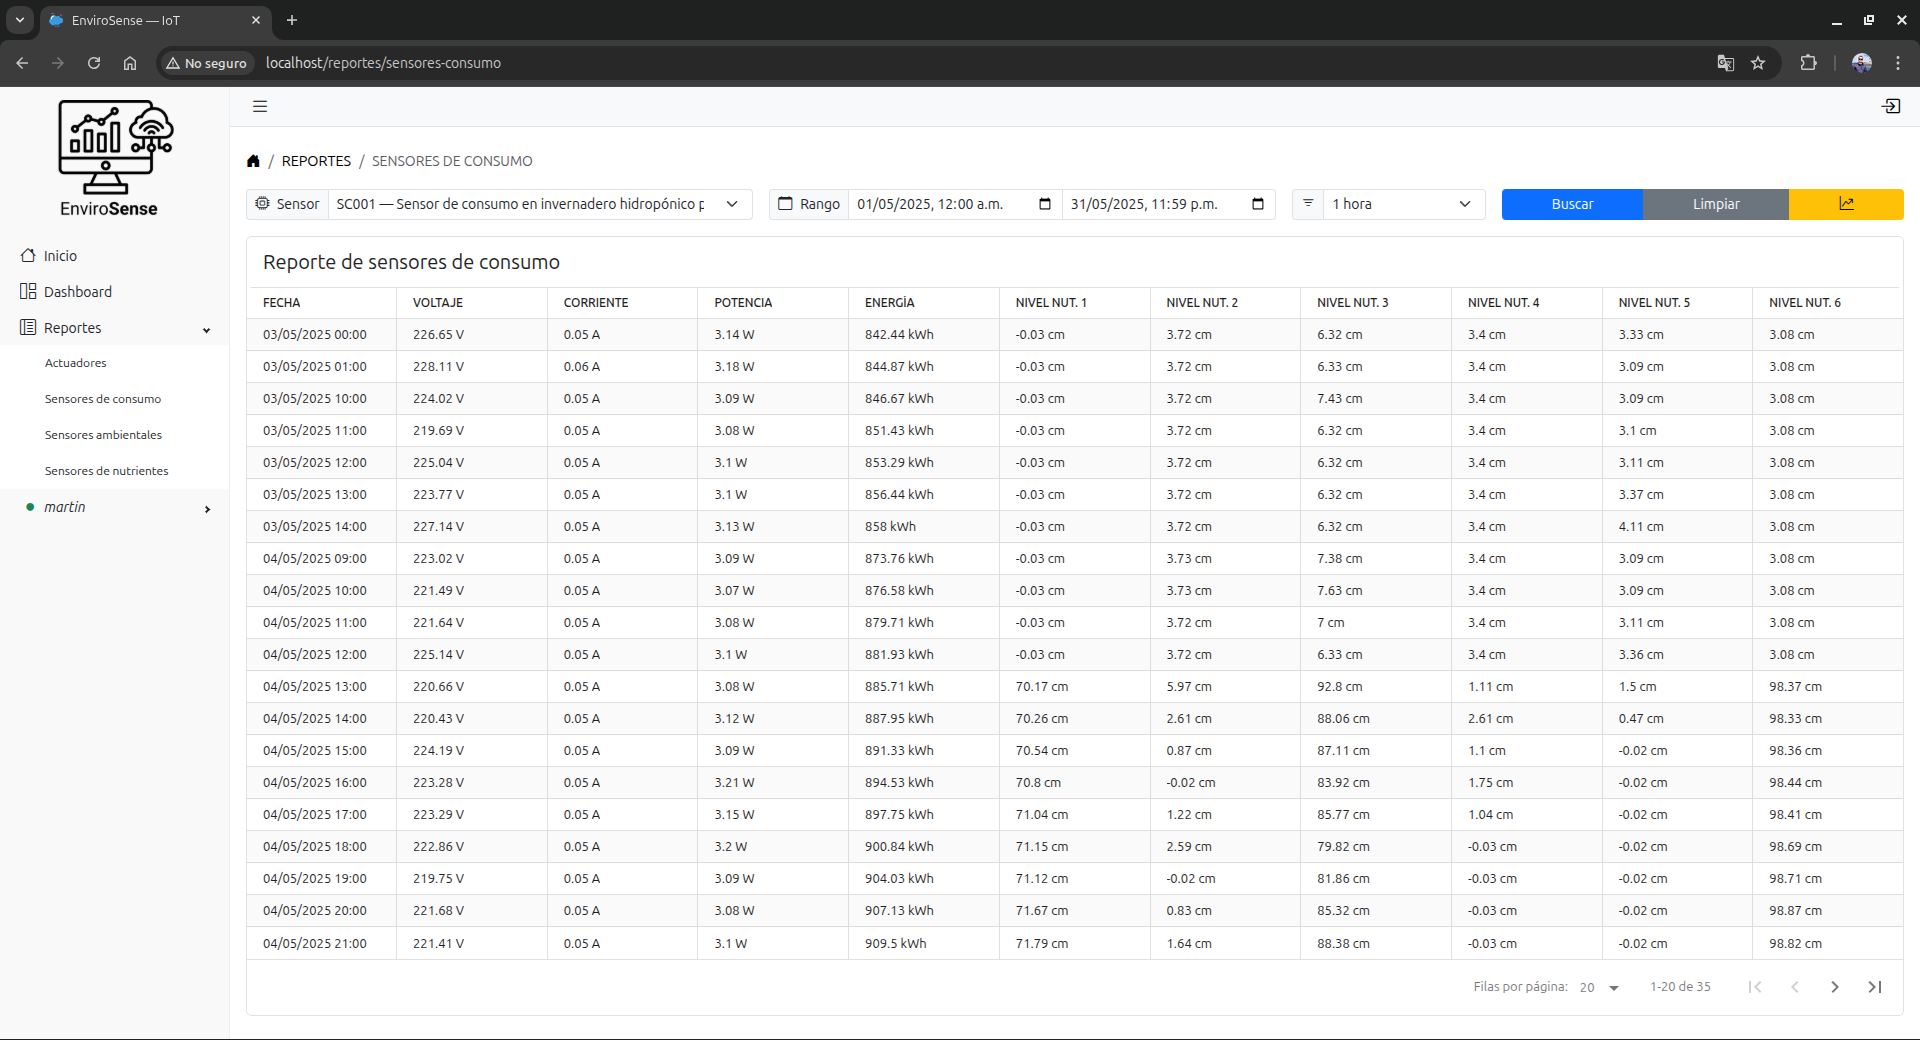
\includegraphics[width=0.99\textwidth]{./Images/28_reportes_1.png}
    \caption{Pantalla de reportes}
    \label{fig:reportes_tabla_consumos}
\end{figure}

La figura \ref{fig:reportes_graficos_consumos} muestra la pantalla de reportes,
donde se exhiben los gráficos con los datos históricos de un sensor de
consumos.

\begin{figure}[H]
    \centering
    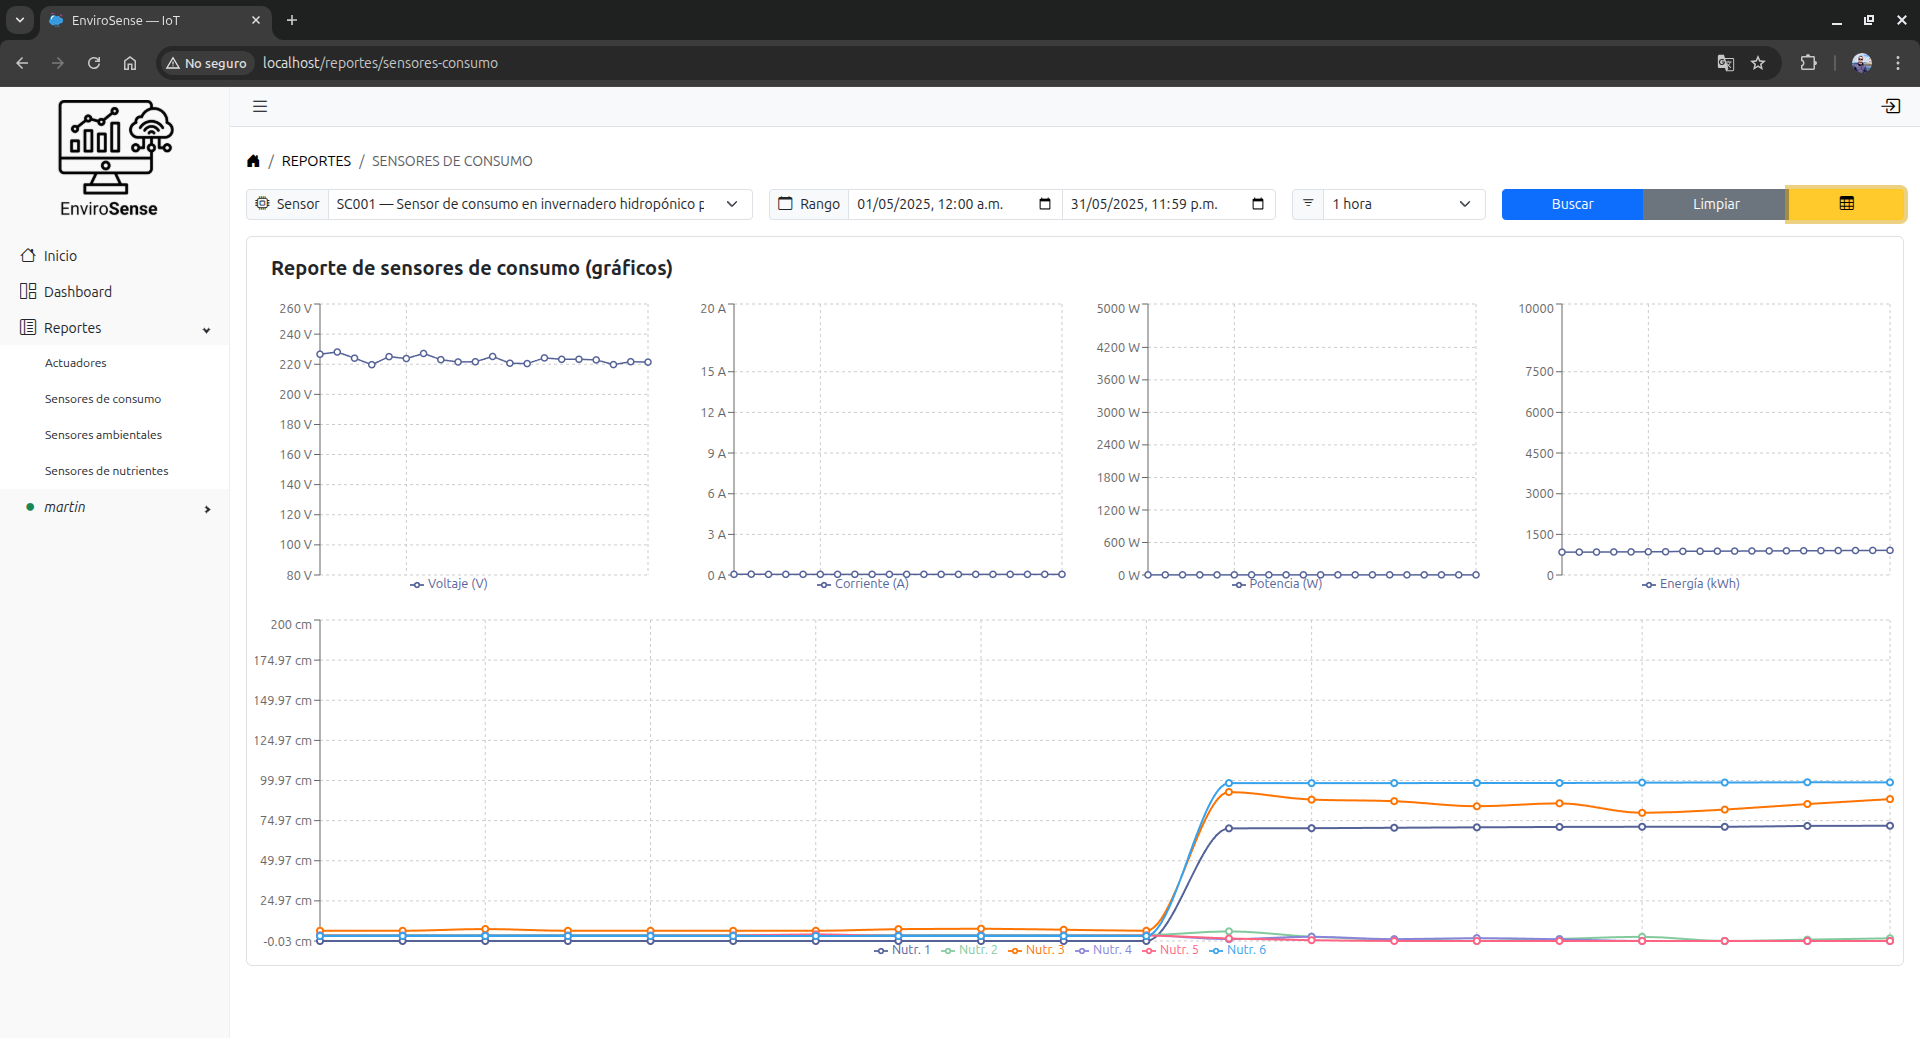
\includegraphics[width=0.99\textwidth]{./Images/28_reportes_2.png}
    \caption{Pantalla de reportes}
    \label{fig:reportes_graficos_consumos}
\end{figure}

La figura \ref{fig:reportes_tabla_actuadores} muestra la pantalla de reportes,
donde se puede observar la tabla con los datos históricos de un actuador.

\begin{figure}[H]
    \centering
    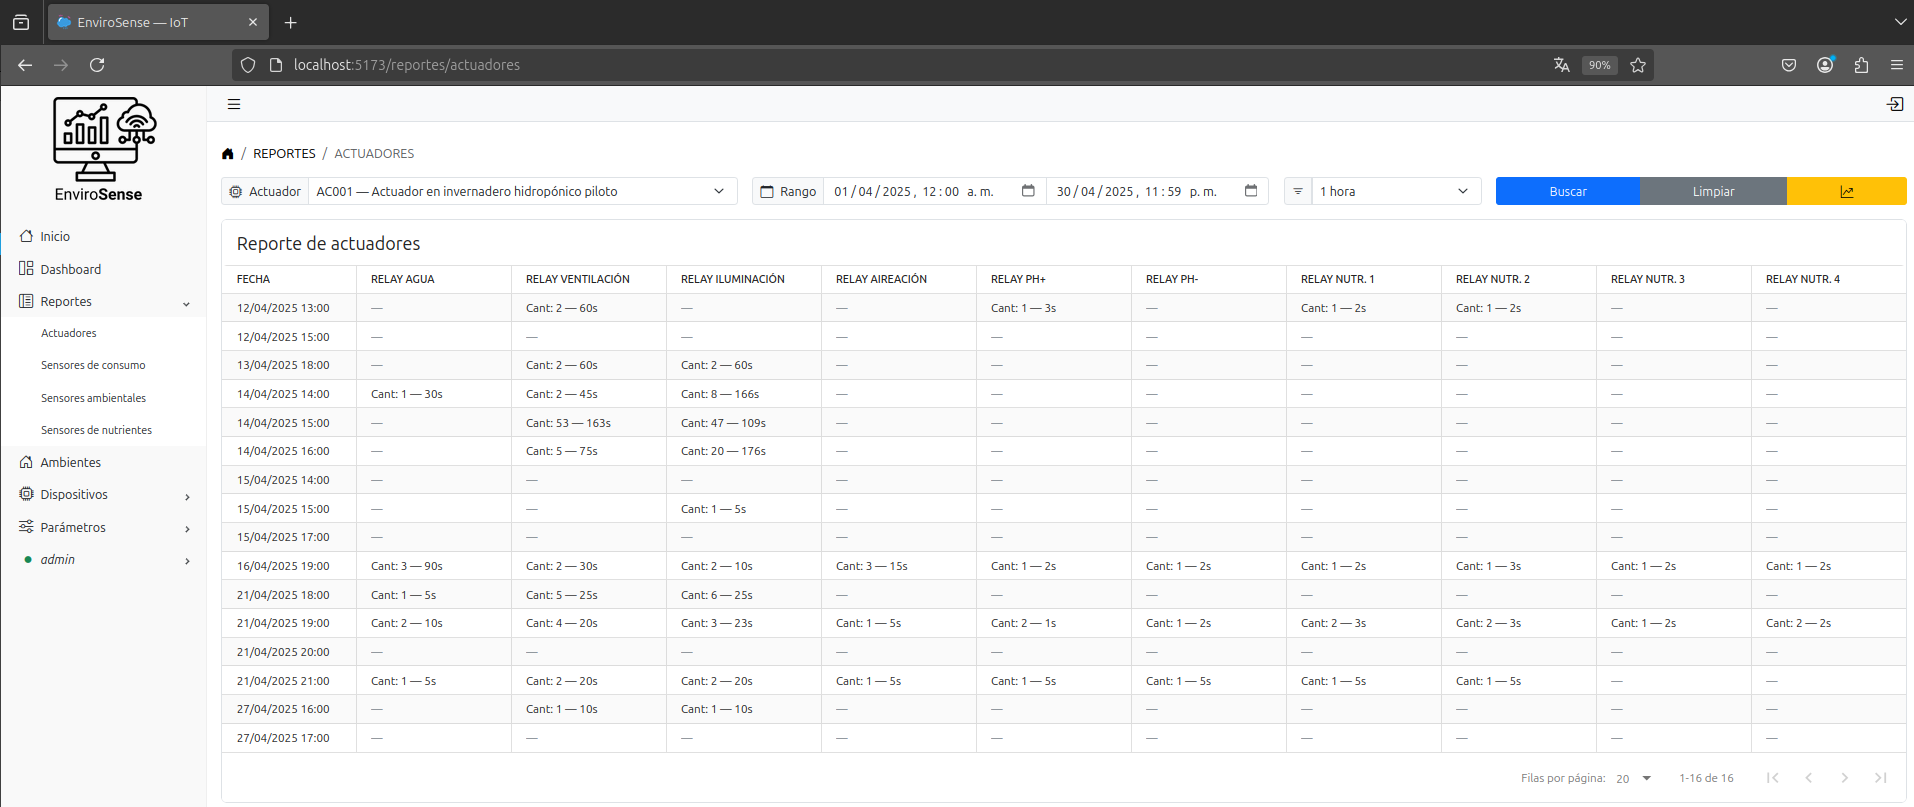
\includegraphics[width=0.99\textwidth]{./Images/28_reportes_3.png}
    \caption{Pantalla de reportes}
    \label{fig:reportes_tabla_actuadores}
\end{figure}

Finalmente, la figura \ref{fig:dashboar_celular} presenta vistas de la
aplicación web en un dispositivo móvil, mosse muestra la pantalla de
visualización de datos en tiempo real. La interfaz se ajusta automáticamente a
distintos tamaños de pantalla, ofreciendo una experiencia de usuario optimizada
en dispositivos móviles y tabletas.

\begin{figure}[H]
    \centering
    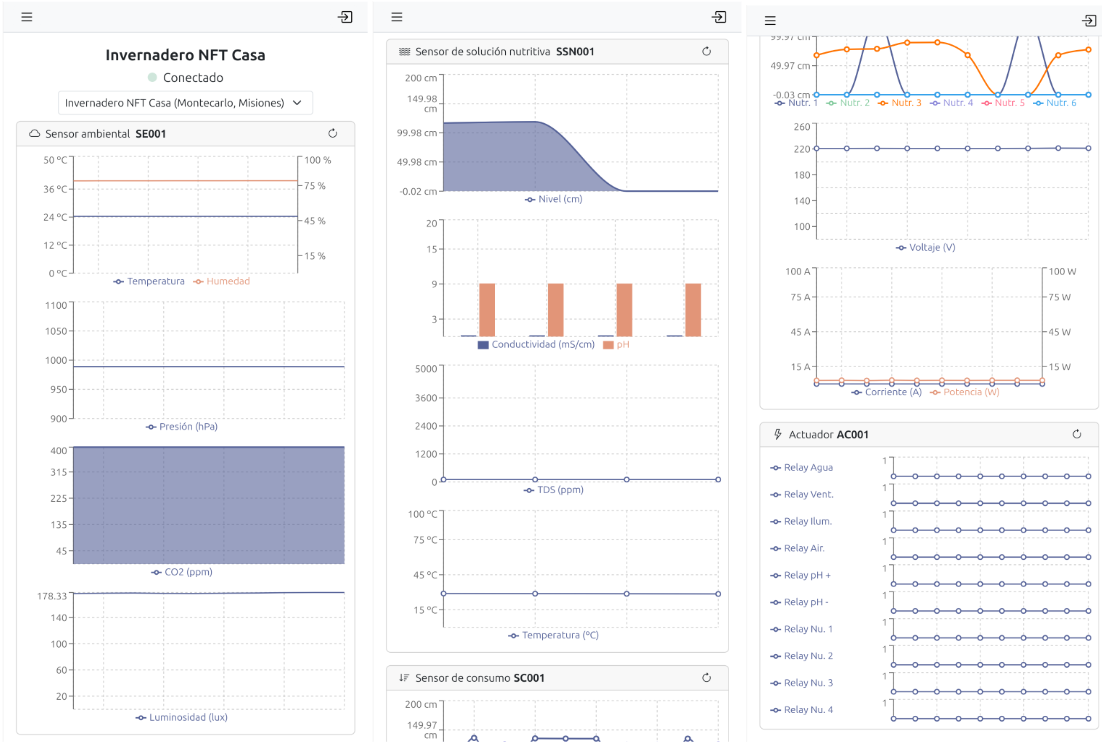
\includegraphics[width=0.99\textwidth]{./Images/29_dashboard_celular.png}
    \caption{Visualización de datos en tiempo real desde un dispositivo móvil}
    \label{fig:dashboar_celular}
\end{figure}

%----------------------------------------------------------------------------------------
%	SECTION 6
%----------------------------------------------------------------------------------------
% \section{Desarrollo de nodos sensores y actuadores}

\section{Desarrollo del firmware de los dispositivos IoT}

En esta sección se detalla el desarrollo del firmware para los nodos 
basados en el microcontrolador ESP32, a través de MicroPython. Se describen las
principales funciones de cada tipo de nodo, la arquitectura del firmware y las
características más relevantes.

\subsection{Arquitectura general del firmware}

Todos los nodos comparten una arquitectura de firmware similar, diseñada para
la adquisición de datos y el control de actuadores, la comunicación
inalámbrica, la gestión de eventos y la interacción con el broker MQTT.

\subsection{Estructura del código}

La estructura general del código para cada nodo se organiza de la siguiente
manera:

\begin{itemize}
    \item \textbf{Importación de librerías}: se importan los módulos necesarios para la
          interacción con los sensores, la comunicación Wi-Fi, la conexión MQTT,
          la gestión del tiempo y otras funcionalidades.
    \item \textbf{Configuración inicial}: se definen las variables y constantes de
          configuración, como los pines de los sensores y relays, los parámetros de conexión
          Wi-Fi y MQTT, y los intervalos de muestreo.
    \item \textbf{Inicialización}: se configuran los periféricos
          del ESP32 y se inicializan los sensores y relays específicos de cada
          tipo de nodo. Se implementan manejos de errores para garantizar la
          robustez del sistema.
    \item \textbf{Funciones auxiliares}: se definen funciones para establecer y chequear
          la conexión Wi-Fi, la sincronización de la hora con un servidor NTP (del
          inglés, \textit{Network Time Protocol}), la carga de certificados TLS y otras
          tareas comunes.
    \item \textbf{Conexión MQTT}: se establece la conexión con el broker MQTT,
          con la utilización de certificados TLS para la seguridad de la comunicación.
    \item \textbf{Callback de mensajes MQTT}: se define una función que se ejecuta cuando
          se reciben mensajes MQTT, esto permite la configuración remota de los nodos
          y la ejecución de acciones específicas.
    \item \textbf{Función de lectura de sensores/control de actuadores}: se implementa
          la lógica específica para leer los datos de los sensores o controlar los
          actuadores.
    \item \textbf{Bucle principal}: se ejecuta un bucle infinito que realiza las
          siguientes tareas de forma continua:
          \begin{itemize}
              \item Verificación de la conexión Wi-Fi.
              \item Lectura de datos de los sensores o control de los actuadores.
              \item Envío de datos al broker MQTT.
              \item Recepción y procesamiento de mensajes MQTT.
              \item Gestión de errores y reinicio del sistema en caso de fallos.
          \end{itemize}
\end{itemize}

\subsection{Gestión de tareas y concurrencia}

Si bien MicroPython no incluye un sistema operativo en tiempo real (RTOS, del
inglés, \textit{Real-Time Operating System}) por defecto, la ejecución
concurrente de tareas se logra mediante la gestión del bucle principal, el uso
de interrupciones y, principalmente, la utilización de los \texttt{Timers} del
ESP32 para la ejecución periódica de tareas.

El firmware desarrollado en los nodos implementa un bucle principal para la
ejecución iterativa de tareas como la conexión Wi-Fi y el procesamiento de
mensajes MQTT.

Para la tarea de activación/desactivación de canales en el nodo actuador se
utilizan los \texttt{Timers} del ESP32, lo que permite descargar esta tarea del
bucle principal y mejorar la eficiencia. Cada tarea se ejecuta con su propio
temporizador, lo que permite ejecutar múltiples tareas de forma simultánea sin
bloquear el bucle principal.

% ----------------------------------------------------------------------------------------

\subsection{Resumen de nodos sensores y actuadores}

En la tabla \ref{tab:nodos_iot} se presenta un resumen de las principales
funciones y de la descripción general del firmware desarrollado para cada uno
de los nodos sensores y actuadores implementados en el sistema. Cada nodo
cumple un rol específico en la adquisición de datos o en el control de
dispositivos, garantizando la comunicación eficiente y segura a través del
protocolo MQTT.

\begin{table}[H]
    \centering
    \caption[Resumen de nodos]{Resumen de nodos: funciones y firmware.}
    % \begin{tabular}{l l l}
    \begin{tabular}{p{1.7cm}p{5.3cm}p{4.9cm}}
        \hline
        \textbf{Nodo}                                     & \textbf{Funciones principales}                                                & \textbf{Descripción del firmware}              \\
        \multirow{6}{1.7cm}{Sensor de consumos}           & Medición de voltaje, corriente y potencia (PZEM-004T)                         & Uso de UART para PZEM-004T                     \\
                                                          & Medición de nivel de líquidos (HC-SR04)                                       & GPIO para HC-SR04                              \\
                                                          & Conexión Wi-Fi                                                                & Envío de datos en formato JSON vía MQTT        \\
                                                          & Configuración remota de intervalo                                             & Sincronización NTP                             \\
                                                          & Indicador LED                                                                 & Manejo de conexión Wi-Fi                       \\
                                                          & Botón de reinicio                                                             & Gestión de errores                             \\
        \hline
        \multirow{7}{1.7cm}{Sensor ambiental}             & Medición de temperatura, humedad y presión (BME280)                           & Comunicación I\textsuperscript{2}C para BME280 \\
                                                          & Medición de luminosidad (BH1750)                                              & UART para MH-Z19C                              \\
                                                          & Medición de concentración de $CO_2$ (MH-Z19C)                                 & Calibración inicial de $CO_2$                  \\
                                                          & Conexión Wi-Fi                                                                & Envío de datos en JSON vía MQTT                \\
                                                          & Configuración remota de intervalo                                             & Sincronización NTP                             \\
                                                          & Indicador LED                                                                 & Reconexión automática Wi-Fi                    \\
                                                          & Botón de reinicio                                                             &                                                \\
        \hline
        \multirow{7}{1.7cm}{Sensor de solución nutritiva} & Medición de temperatura (DS18B20)                                             & Lectura OneWire para DS18B20                   \\
                                                          & Medición de pH, CE y TDS                                                      & Medición de CE/TDS/pH                          \\
                                                          & Medición de nivel de líquidos (HC-SR04)                                       & Promedio de muestras                           \\
                                                          & Conexión Wi-Fi                                                                & Envío de datos en JSON vía MQTT                \\
                                                          & Configuración remota de intervalo                                             & Sincronización NTP                             \\
                                                          & Indicador LED                                                                 & Manejo de errores                              \\
                                                          & Botón de reinicio                                                             &                                                \\
        \hline
        \multirow{7}{1.7cm}{Actuador}                     & Control de relés para dispositivos (bombas, aireadores, luces, dosificadores) & Control de salidas GPIO                        \\
                                                          & Ejecución simultánea de comandos                                              & Recepción de comandos MQTT                     \\
                                                          & Conexión Wi-Fi                                                                & Ejecución de temporizadores con Timers ESP32   \\
                                                          & Configuración remota                                                          & Manejo de estados de relés en JSON             \\
                                                          & Indicador LED                                                                 & Sincronización NTP                             \\
                                                          & Botón de reinicio                                                             & Reconexión Wi-Fi automática                    \\
        \hline
    \end{tabular}
    \label{tab:nodos_iot}
\end{table}
% ----------------------------------------------------------------------------------------

\subsection{Comunicación inalámbrica}

Todos los nodos utilizan la comunicación Wi-Fi para conectarse al broker MQTT.

\subsubsection{Wi-Fi}

Se utiliza de base la librería \texttt{wifi\_manager}
\cite{MicroPythonWifiManager} para facilitar la conexión y gestión de la red
Wi-Fi. Los nodos intentan conectarse a la red Wi-Fi configurada y realizan
verificaciones periódicas de la conexión para garantizar la disponibilidad de
la red. Se realizan cambios en la librería para adaptarla a las necesidades del
trabajo, como leer SSID con espacios en blanco y se incorpora un campo de tipo
menú desplegable para seleccionar una zona horaria.

\subsubsection{MQTT}

Se utiliza la librería \texttt{umqtt.robust} de \texttt{MicropythonLib}
\cite{MicropythonLib} para implementar un cliente MQTT, capaz de reconectarse
automáticamente al broker en caso de fallos de conexión. Se implementa TLS para
la seguridad de la comunicación, utilizando certificados almacenados en el
dispositivo.

\subsubsection{Protocolo de comunicación}

Los datos de los sensores y los comandos de control se transmiten en formato
JSON a través de los tópicos MQTT definidos en el archivo \texttt{config.py}.
Se utiliza un esquema de mensajes estandarizado para facilitar el procesamiento
de los datos en el sistema central.

% ----------------------------------------------------------------------------------------

\subsection{Gestión de la configuración}

La configuración de los nodos, código del sensor o actuador, tópicos MQTT, el
intervalo de muestreo y los parámetros de conexión Wi-Fi, se almacena en
archivos locales en el ESP32. Esto permite la persistencia de la configuración
entre reinicios.

\subsubsection{Archivo de configuración}

El archivo \texttt{config.py} contiene constantes y variables de configuración
específicas de cada nodo. Incluye:

\begin{itemize}
    \item \textbf{Códigos de identificación}: incluye el código para identificar unívocamente
          a cada dispositivo.
    \item \textbf{Tópicos MQTT}: incluye los tópicos para la publicación y
          suscripción de datos. Cada nodo tiene un tópico único para enviar datos
          y otro para recibir comandos.
    \item \textbf{Parámetros de conexión AWS IoT Core}: incluye el identificador del cliente y el
          endpoint del broker MQTT.
\end{itemize}
% ----------------------------------------------------------------------------------------

\subsection{Comunicación inalámbrica}

Todos los nodos utilizan la comunicación Wi-Fi para conectarse al broker MQTT.

\subsubsection{Wi-Fi}

Se utiliza de base la librería \texttt{wifi\_manager}
\cite{MicroPythonWifiManager} para facilitar la conexión y gestión de la red
Wi-Fi. Los nodos intentan conectarse a la red Wi-Fi configurada y realizan
verificaciones periódicas de la conexión para garantizar la disponibilidad de
la red. Se realizan cambios en la librería para adaptarla a las necesidades del
trabajo, como leer SSID con espacios en blanco y se incorpora un campo de tipo
menú desplegable para seleccionar una zona horaria.

\subsubsection{MQTT}

Se utiliza la librería \texttt{umqtt.robust} de \texttt{MicropythonLib}
\cite{MicropythonLib} para implementar un cliente MQTT, capaz de reconectarse
automáticamente al broker en caso de fallos de conexión. Se implementa TLS para
la seguridad de la comunicación, utilizando certificados almacenados en el
dispositivo.

\subsubsection{Protocolo de comunicación}

Los datos de los sensores y los comandos de control se transmiten en formato
JSON a través de los tópicos MQTT definidos en el archivo \texttt{config.py}.
Se utiliza un esquema de mensajes estandarizado para facilitar el procesamiento
de los datos en el sistema central.

% ----------------------------------------------------------------------------------------

\subsection{Gestión de la configuración}

La configuración de los nodos, código del sensor o actuador, tópicos MQTT, el
intervalo de muestreo y los parámetros de conexión Wi-Fi, se almacena en
archivos locales en el ESP32. Esto permite la persistencia de la configuración
entre reinicios.

\subsubsection{Archivo de configuración}

El archivo \texttt{config.py} contiene constantes y variables de configuración
específicas de cada nodo. Incluye:
\begin{itemize}
    \item \textbf{Códigos de identificación}: incluye el código para identificar unívocamente
          a cada dispositivo.
    \item \textbf{Tópicos MQTT}: incluye los tópicos para la publicación y
          suscripción de datos. Cada nodo tiene un tópico único para enviar datos
          y otro para recibir comandos.
    \item \textbf{Parámetros de conexión AWS IoT Core}: incluye el identificador del cliente y el
          endpoint del broker MQTT.
\end{itemize}

\subsubsection{Archivo de configuración del intervalo}

El intervalo de muestreo de los sensores se guarda en el archivo
\texttt{interval.conf}. Al inicio del programa, se intenta leer el valor del
intervalo desde este archivo. Si el archivo no existe o está corrupto, se
utiliza un valor por defecto. Los mensajes MQTT pueden modificar este
intervalo, y el nuevo valor se guarda en el archivo para su uso en futuros
reinicios.

\subsubsection{Archivo de configuración Wi-Fi}

Los parámetros de conexión Wi-Fi (SSID y contraseña) se almacenan en el archivo
\texttt{wifi.dat}. Esto permite que el nodo se reconecte automáticamente a la
red Wi-Fi después de un reinicio. Este archivo permite almacenar múltiples
configuraciones de red, lo que facilita la conexión a diferentes redes Wi-Fi en
diferentes ubicaciones.

En caso de que el nodo no pueda conectarse a la red Wi-Fi, se activa un
servidor web, que permite al usuario configurar la red Wi-Fi a la que desea
conectarse. Este servidor web se ejecuta en el ESP32 y proporciona una interfaz
de usuario simple para seleccionar el SSID, ingresar la contraseña de la red y
seleccionar la zona horaria. Una vez que el usuario ingresa la información
necesaria, el nodo intenta conectarse a la red Wi-Fi especificada. Si la
conexión es exitosa, se guarda la configuración en el archivo \texttt{wifi.dat}
y el nodo se reinicia para aplicar la nueva configuración.

\subsubsection{Archivo de configuración de la zona horaria}

La zona horaria se lee desde el archivo \texttt{timezone.conf} para permitir la
correcta conversión de las marcas de tiempo.

% ----------------------------------------------------------------------------------------

\subsection{Manejo de errores}

Se implementan mecanismos de manejo de errores en todo el firmware para
garantizar la robustez y la confiabilidad de los nodos.

\subsubsection{Manejo de excepciones}

Se utilizan bloques \texttt{try-except} para capturar y manejar excepciones que
pueden ocurrir durante la ejecución del programa. Esto permite que el programa
continúe funcionando incluso si se produce un error, como un fallo en la
lectura de un sensor o un problema de conexión de red.

\subsubsection{Reintentos}

En algunas operaciones críticas, como la conexión Wi-Fi y la sincronización de
la hora con el servidor NTP, se implementan mecanismos de reintento. Si la
operación falla inicialmente, el programa intentará realizarla nuevamente un
número determinado de veces antes de darla por fallida.

\subsubsection{Reinicios}

En caso de errores irrecuperables, el programa puede reiniciar el ESP32. Esto
permite que el nodo se recupere de situaciones en las que no puede seguir
funcionando correctamente.

\subsubsection{Logging}

Se utilizan mensajes de registro (\texttt{print}) para informar sobre el estado
del programa y los errores que se producen. Esto facilita la depuración y el
mantenimiento del firmware.

\subsubsection{Optimización de recursos}

Se utiliza la función \texttt{gc.collect()} para liberar memoria
periódicamente. Esto ayuda a prevenir problemas de memoria insuficiente,
especialmente en aplicaciones que se ejecutan durante largos períodos de
tiempo.

%----------------------------------------------------------------------------------------
%	SECTION 7
%----------------------------------------------------------------------------------------
\section{Despliegue del sistema}

% Esta sección describe el proceso de implementación y configuración del sistema
% en el entorno de prueba.